\documentclass[11pt]{article}

\usepackage[a4paper,margin=1in]{geometry}
\setlength{\emergencystretch}{4.5em}
\usepackage[T1]{fontenc}

\usepackage[utf8]{inputenc}
\usepackage[expansion=false]{microtype}
\usepackage{amsmath,amssymb,amsthm}
\usepackage{booktabs}
\usepackage{array}
\usepackage{tabularx}
\usepackage{xcolor}
\usepackage[numbers,sort&compress]{natbib}
\usepackage{pgfplots}
\pgfplotsset{compat=1.16}
\usetikzlibrary{arrows.meta,positioning}
\usepackage{url}
\usepackage[colorlinks=true,linkcolor=blue!50!black,citecolor=blue!50!black,urlcolor=blue!60!black]{hyperref}

% ---------------------------------------------------------------------------
% Footer: DOI on every page (incl. the title page's plain style)
% ---------------------------------------------------------------------------
\usepackage{fancyhdr}
\newcommand{\paperdoi}{10.5281/zenodo.20787816}
\newcommand{\doifooter}{\footnotesize DOI:~\href{https://doi.org/\paperdoi}{\paperdoi}}
\pagestyle{fancy}
\fancyhf{}
\renewcommand{\headrulewidth}{0pt}
\fancyfoot[C]{\thepage}
\fancyfoot[R]{\doifooter}
\fancypagestyle{plain}{%
  \fancyhf{}%
  \renewcommand{\headrulewidth}{0pt}%
  \fancyfoot[C]{\thepage}%
  \fancyfoot[R]{\doifooter}%
}

% ---------------------------------------------------------------------------
% Helper macros
% ---------------------------------------------------------------------------
\newcommand{\code}[1]{\texttt{#1}}


\newtheorem{definition}{Definition}
\newtheorem{remark}{Remark}

\newcolumntype{Y}{>{\raggedright\arraybackslash}X}

% Measured numbers for the executable instance (Section~\ref{sec:caseD}),
% generated by src/A/evidence/measure_squeeze.py -- never hand-edited.
\IfFileExists{macros/results.tex}{% GENERATED by src/A/evidence/measure_squeeze.py -- do not hand-edit.
% Re-run that script to regenerate. Every Use-Case-A number traces here.
\newcommand{\ResAblationBarrierOff}{0}
\newcommand{\ResAblationBarrierOn}{5}
\newcommand{\ResAblationSeeded}{5}
\newcommand{\ResWorkedCertifiedMetrics}{24}
\newcommand{\ResWorkedClauses}{5}
\newcommand{\ResWorkedDefectsCaught}{5}
\newcommand{\ResWorkedDetectionPct}{100\%}
\newcommand{\ResWorkedMetrics}{2}
\newcommand{\ResWorkedPositiveCells}{8}
\newcommand{\ResWorkedSeededDefects}{5}
\newcommand{\ResWorkedThreeWayAgree}{8}
\newcommand{\ResWorkedWarehouseEvents}{291}
\newcommand{\ResWorkedWarehouseUsers}{50}
}{}
\IfFileExists{macros/results_b.tex}{% GENERATED by src/B/evidence/measure_squeeze.py -- do not hand-edit.
\newcommand{\ResBArchiveCases}{6}
\newcommand{\ResBBarrierOff}{0}
\newcommand{\ResBBarrierOn}{4}
\newcommand{\ResBClauses}{3}
\newcommand{\ResBDefectsCaught}{4}
\newcommand{\ResBDetectionPct}{100\%}
\newcommand{\ResBScenarios}{5}
\newcommand{\ResBSeededDefects}{4}
}{}
\IfFileExists{macros/results_c.tex}{% GENERATED by src/C/evidence/measure_squeeze.py -- do not hand-edit.
\newcommand{\ResCBarrierOff}{0}
\newcommand{\ResCBarrierOn}{4}
\newcommand{\ResCClauses}{3}
\newcommand{\ResCDefectsCaught}{4}
\newcommand{\ResCDetectionPct}{100\%}
\newcommand{\ResCLegacyRoutes}{2}
\newcommand{\ResCSeededDefects}{4}
\newcommand{\ResCTestCases}{5}
}{}
\IfFileExists{macros/results_d.tex}{% GENERATED by verify/results_d.py -- do not hand-edit.
\newcommand{\ResDBarrierOff}{0}
\newcommand{\ResDClauses}{3}
\newcommand{\ResDDefectsCaught}{2}
\newcommand{\ResDDetectionPct}{100\%}
\newcommand{\ResDSeededDefects}{2}
}{}
\IfFileExists{macros/coupling.tex}{% GENERATED by verify/coupling_measure.py -- do not hand-edit.
\newcommand{\ResCouplingA}{2.6\%}
\newcommand{\ResCouplingAval}{2.6}
\newcommand{\ResCouplingB}{0.7\%}
\newcommand{\ResCouplingBval}{0.7}
\newcommand{\ResCouplingC}{1.4\%}
\newcommand{\ResCouplingCval}{1.4}
}{}
\IfFileExists{macros/synthesis.tex}{% GENERATED by verify/synthesis.py -- do not hand-edit.
\newcommand{\ResAllBarrierOff}{0}
\newcommand{\ResAllCaught}{15}
\newcommand{\ResAllSeeded}{15}
\newcommand{\ResNArchetypes}{3}
\newcommand{\ResNTerrains}{4}
}{}
\IfFileExists{macros/eval.tex}{% GENERATED by verify/eval_protocol.py -- do not hand-edit.
\newcommand{\ResEvalConfigsPending}{3}
\newcommand{\ResEvalConfigsRunnable}{2}
\newcommand{\ResEvalHypMeasured}{1}
\newcommand{\ResEvalHypPending}{3}
\newcommand{\ResEvalHypTotal}{4}
}{}
\IfFileExists{macros/pilot.tex}{% GENERATED by eval/pilot/score.py -- do not hand-edit.
\newcommand{\ResPilotDetectionOff}{4}
\newcommand{\ResPilotDetectionOn}{4}
\newcommand{\ResPilotTasks}{4}
\newcommand{\ResPilotValidityOff}{100}
\newcommand{\ResPilotValidityOn}{100}
}{}
\IfFileExists{macros/pilot2.tex}{% GENERATED by eval/pilot2/score.py -- do not hand-edit.
\newcommand{\ResPilotTwoBuggy}{0}
\newcommand{\ResPilotTwoIndepCaught}{0}
\newcommand{\ResPilotTwoSelfCaught}{0}
\newcommand{\ResPilotTwoTasks}{4}
}{}
\IfFileExists{macros/pilot3.tex}{% GENERATED by eval/pilot3/score.py -- do not hand-edit.
\newcommand{\ResPilotThreeBuggy}{0}
\newcommand{\ResPilotThreeIndepStrong}{0}
\newcommand{\ResPilotThreeIndepWeak}{0}
\newcommand{\ResPilotThreeSelf}{0}
\newcommand{\ResPilotThreeTasks}{5}
}{}
\IfFileExists{macros/study.tex}{% GENERATED by eval/study/score.py -- do not hand-edit.
\newcommand{\ResStudyBuggy}{0}
\newcommand{\ResStudyDiscIndep}{0}
\newcommand{\ResStudyDiscSelf}{0}
\newcommand{\ResStudyImpls}{24}
\newcommand{\ResStudyIndepCaught}{0}
\newcommand{\ResStudyP}{1.000}
\newcommand{\ResStudySelfCaught}{0}
}{}
\IfFileExists{macros/swebench.tex}{% GENERATED by eval/swebench/run_protocol.py -- do not hand-edit.
\newcommand{\ResSweFailTests}{35}
\newcommand{\ResSweInstances}{15}
\newcommand{\ResSweRepos}{2}
\newcommand{\ResSweStepsPending}{3}
\newcommand{\ResSweStepsRunnable}{2}
}{}
\IfFileExists{macros/reflexive.tex}{% GENERATED by verify/reflexive_measures.py -- do not hand-edit.
\newcommand{\ResReflexCiteRows}{46}
\newcommand{\ResReflexDefects}{8}
\newcommand{\ResReflexDefectsEvid}{4}
\newcommand{\ResReflexDefectsLit}{4}
\newcommand{\ResReflexGapDocs}{2}
\newcommand{\ResReflexRecords}{51}
\newcommand{\ResReflexRecordsFull}{43}
\newcommand{\ResReflexResultRows}{38}
\newcommand{\ResReflexSpecDocs}{78}
\newcommand{\ResReflexTerrains}{4}
}{}
\IfFileExists{macros/levelup.tex}{% GENERATED by verify/levelup_measures.py -- do not hand-edit.
\newcommand{\ResLevelupADiverge}{30}
\newcommand{\ResLevelupCBlend}{50}
\newcommand{\ResLevelupCycles}{10}
\newcommand{\ResLevelupDMax}{20}
\newcommand{\ResLevelupDMin}{14}
\newcommand{\ResLevelupDNotFound}{19}
\newcommand{\ResLevelupDistinctMax}{7}
\newcommand{\ResLevelupPool}{100}
\newcommand{\ResLevelupSample}{20}
\newcommand{\ResLevelupTerrains}{4}
}{}
\IfFileExists{macros/calibration.tex}{% GENERATED by verify/flag_rate.py -- do not hand-edit.
\newcommand{\ResCalibMonitors}{3}
\newcommand{\ResCalibExternalCatches}{1}
\newcommand{\ResCalibDefects}{8}
\newcommand{\ResCalibRouted}{13}
\newcommand{\ResCalibClaims}{85}
\newcommand{\ResCalibHistory}{5}
}{}
\IfFileExists{macros/gates.tex}{% GENERATED by verify/gate_s_measures.py -- do not hand-edit.
\newcommand{\ResGateSFlagged}{2}
\newcommand{\ResGateSInstances}{4}
\newcommand{\ResGateSSkills}{19}
}{}
\IfFileExists{macros/skill.tex}{% GENERATED by verify/skill_measures.py -- do not hand-edit.
\newcommand{\ResSkillBClasses}{8}
\newcommand{\ResSkillBErrFirst}{2.9}
\newcommand{\ResSkillCycles}{100}
\newcommand{\ResSkillDPool}{100}
\newcommand{\ResSkillDTactics}{2}
\newcommand{\ResSkillDWall}{16}
\newcommand{\ResSkillInstances}{4}
\newcommand{\ResSkillLearned}{19}
\newcommand{\ResSkillMaxSolvableLast}{0}
}{}
\IfFileExists{macros/realworld.tex}{% Numbers for the real-world application (Section~\ref{sec:realworld}).
% TRANSCRIBED from the run's on-disk artifacts under real-use-case/ -- there is no
% measurement harness emitting these (the experiment used cargo creusot directly via
% Bash, not a macro-emitting script), so each macro carries the artifact it comes from
% and Gate~C re-derives it against that artifact. Do not hand-edit to a value the
% artifact does not show.
%
% Sources:
%   real-use-case/lace-attack-surface.md      (ROBUST / PARTIAL / BLOCKED counts)
%   real-use-case/lace-issues/README.md       (the four defects; how found)
%   real-use-case/lace-claims-validation.md   (the unsafe-site counts)
%   real-use-case/report.md                   (the warm-up corpus run)
%
% --- the four real defects (lace-issues/README.md) ---
\newcommand{\ResRWBugs}{four}
\newcommand{\ResRWBugsNum}{4}
\newcommand{\ResRWBugsVC}{three}          % found as unproved Creusot VCs (ISSUE-1..3)
\newcommand{\ResRWBugsCallGraph}{one}     % found by call-graph analysis (ISSUE-4)
%
% --- coverage of the untrusted-input attack surface (lace-attack-surface.md) ---
\newcommand{\ResRWRobust}{25}             % input-facing functions proven ROBUST
\newcommand{\ResRWRobustPOne}{8}          % priority-1 (disk/ESP)
\newcommand{\ResRWRobustPTwo}{17}         % priority-2 (peripheral/firmware/derived)
\newcommand{\ResRWInputFns}{38}           % ~38 input-facing functions targeted
\newcommand{\ResRWPartial}{2}             % panic-safe, residual is SMT incompleteness
\newcommand{\ResRWBlocked}{6}             % blocked by creusot-std modeling gaps
%
% --- reconciled disposition (sum of the four disjoint categories above) ---
% Robust(25) + defect-bearing(4) + blocked(6) + partial(2) = 37 verdict-slots. The
% categories are disjoint EXCEPT ISSUE-4 (the recursion, found by call-graph) lies in a
% BLOCKED file, so it is counted once as defect-bearing and once as blocked: 37 slots
% over 36 DISTINCT functions. (ResRWInputFns=38 above was the loosely-counted "targeted"
% figure -- leaf helpers/iterators counted as rows; the reconciled per-verdict count is 36.)
\newcommand{\ResRWVerdictSlots}{37}
\newcommand{\ResRWDistinctFns}{36}
% --- the warm-up corpus run (report.md) ---
\newcommand{\ResRWCorpusFiles}{241}
\newcommand{\ResRWCorpusProved}{74}
\newcommand{\ResRWCorpusPartial}{8}
\newcommand{\ResRWCorpusFailed}{6}
\newcommand{\ResRWCorpusTrivial}{153}
% \ResRWFabCaught retired: the 10-fabrication warm-up count was a skill-training exercise,
% not a paper result. The faithfulness-gate MECHANISM (a fabricated proof cannot survive a
% strip-and-recompile check) is kept in prose; the count is deliberately not reported.
%
% --- a static structural claim re-checked (lace-claims-validation.md, claim 5) ---
\newcommand{\ResRWUnsafePlatform}{77}
\newcommand{\ResRWUnsafeUtil}{5}
\newcommand{\ResRWUnsafeStubble}{3}
\newcommand{\ResRWUnsafeSpeedboot}{0}
}{}

% ---------------------------------------------------------------------------
\title{\textbf{The Squeeze Loop Strategy:}\\
\Large Catching Coherent-and-Wrong Artifacts with an Author-Independent Executable Oracle}

\author{%
  Fabrice Derepas\\[2pt]
  Canonical\\[2pt]
  \url{https://github.com/canonical/squeeze-loop}%
}
\date{June 2026}

\begin{document}
\maketitle

\begin{abstract}
Agentic large language model (LLM) workflows increasingly run in \emph{loops}: one agent
produces, another critiques or tests, and the cycle repeats until an acceptance signal
fires. They fail in one characteristic way. When that signal is producible --- or even
merely visible --- to the agent being judged, the loop converges on agreement with itself
rather than on correctness. We call the result \emph{coherent-and-wrong}: an artifact that
passes its own checks while missing the intended property. Self-preference, sycophancy, and
tests tuned to the code are all this shape.

The \emph{squeeze loop strategy} removes that failure's root condition by construction wherever an
author-independent executable oracle exists. Every actor is pinned between a soft \emph{upper bound} ---
a citable authority, the strongest claim it may make --- and a hard, executable \emph{lower bound} it
cannot alter; it answers to a \emph{different} authority pair from every other (the \emph{disjointness
principle}), and a judging actor never sees the implementation it grades. Where no oracle exists, the
loop closes instead by nesting that terminates in human review.

This is a methods paper; stripped of the apparatus, its evidence establishes three things. \emph{First,
an LLM's proof can be made trustworthy by a mechanical check.} Applied unchanged to an external UEFI
bootloader (Canonical's \code{lace}), a \emph{faithfulness gate} strips every annotation the agent added
and demands the original source back byte-for-byte --- a cheated proof cannot survive --- and under it
the loop proved \ResRWRobust{} functions robust and found \ResRWBugsNum{} real security bugs, with no
human judgment and no detection rate to tune. \emph{Second, when a spec genuinely contradicts itself, a
smarter model does not help and can hurt.} On a balanced authority conflict the error \emph{rose} with
model size ($0.54\!\to\!1.00$), every model-based check (self-critique, a second model, a different
provider) reproduced the same wrong reading from shared priors, and only an executable ground truth
caught it. \emph{Third, the mechanism the strategy is built around --- hiding the implementation from the judge so
it cannot anchor --- does not measurably matter}: across $504$ trials its outcome effect never appeared,
because a competent model handed an explicit authority simply follows it. The unifying claim those support: what
catches a fluent-but-wrong artifact is an \emph{independent executable check} --- not a smarter model,
not more agents, not hiding the code from the judge. Four executable seeded instances over three terrains (analytics and Rocq proofs, a refund
agent, an API guard) demonstrate that the construction instantiates and its gate fires on each ---
existence demonstrations, not efficacy measurements, so a powered comparison remains future work.
\end{abstract}

% ===========================================================================
\section{Introduction}
\label{sec:intro}

The unit of progress in applied LLM systems is shifting from the single
completion to the \emph{loop}: plan--act--observe cycles
\citep{yao2022react,wang2023voyager}, generate--critique--refine cycles
\citep{madaan2023selfrefine,shinn2023reflexion}, and multi-agent pipelines in
which differentiated roles (programmer, tester, reviewer, product manager)
pass artifacts to one another until the work is declared done
\citep{li2023camel,wu2023autogen,hong2023metagpt,qian2023chatdev}. The promise
is division of labor; the recurring disappointment is a particular failure
shape. When the signal that terminates the loop can be produced, edited, or
simply \emph{seen} by the actor whose work it judges, the loop converges not on
correctness but on agreement with itself. The empirical literature documents
several faces of this failure: intrinsic self-correction that does not correct
\citep{huang2023cannot}, evaluators that recognize and favor their own
generations \citep{panickssery2024llm}, judges with systematic position and
verbosity biases \citep{zheng2023judging}, and models that yield to the user's
framing rather than the evidence \citep{sharma2023sycophancy}. At the level of
a whole workflow, this is Goodhart's law in organizational form
\citep{manheim2018goodhart,krakovna2020specification,amodei2016concrete}: the
acceptance signal is a proxy. Any actor able to influence its own proxy will,
under optimization pressure, satisfy the proxy rather than the target.

This paper describes a strategy for operating a set of agents so that the
failure shape above is excluded \emph{by construction} on the executable side
rather than discouraged by instruction. We call it the \emph{squeeze loop
strategy}. We scope the phrase \emph{by construction}: against the hard,
executable lower bound the failure's root condition is removed structurally,
with no judge in the loop; the soft, editorial side carries no such mechanical
guarantee at a single level and is instead closed by \emph{nesting} --- an
outer squeeze holding a disjoint $(U,L)$ pair over the inner coordinator ---
terminating in a human or external reviewer (\S\ref{sec:strategy}). Its two
central ideas are simple to state:

\begin{enumerate}
\item \textbf{The squeeze.} Every actor is held between two constraints it
  does not control: an \emph{upper bound} --- a citable normative authority
  fixing the strongest claim the actor may make --- and a \emph{lower bound}
  --- an executable ground truth whose verdict the actor cannot alter. A
  deliverable is admissible only in the band between the two; the actor's
  freedom is exactly the width of that band.
\item \textbf{Disjointness.} Every actor answers to a \emph{different} pair of
  authorities, and the pairs are chosen so that their intersection is the
  correct deliverable while no single actor's evidence base is sufficient on
  its own. Each actor's characteristic failure mode is therefore caught by a
  different actor that cannot share its blind spot; correctness is the fixed
  point that satisfies all squeezes simultaneously.
\end{enumerate}

The \emph{loop} is the protocol that circulates work through the band: forward
through plan documents under a status handshake
(\code{DRAFT} $\rightarrow$ editorial \code{APPROVED} $\rightarrow$
\code{DONE}), backward through \emph{gap documents} that reopen an item on any
divergence, with \emph{done} defined exclusively by machine-checked gates ---
never by an agent's report of success.

A concrete case makes the shape vivid. A revenue metric is to be computed, and the
handbook mandates \emph{net} revenue (gross minus refunds). An implementer instead
computes \emph{gross}: a single, internally consistent program that runs, returns a
plausible number, and passes every check it can see, including its own tests. That is
coherent-and-wrong: fluent, self-certifying, off. The squeeze catches it not with a
better test but by \emph{who holds what}. An independent exerciser, given only the
handbook and never the implementation, derives the \emph{net} figure; the two disagree
at the acceptance gate. The implementer cannot relieve the constraint, never having held
the exerciser's authority; the exerciser cannot be fooled by the same blind spot, never
having seen the gross-revenue code. We return to this instance, measured, in
Section~\ref{sec:caseD}.

The strategy was developed and operated, not designed on paper. It emerged from running
coordinator--worker loops of LLM coding agents, and we instantiate it here as four
\emph{executable, reproducible} instances over three \emph{epistemic terrains}: one where an
external specification already says what correct is (carrying two instances: tabular analytics
and machine-checked proofs); one where no external authority exists for the property at all; and
one where the meaning of every construct splits across two planes with separate authorities. The
topology stays fixed while the squeeze is rebuilt from different materials each time, every
number from a re-runnable harness (Section~\ref{sec:archetypes}). This is a methods paper: it
contributes the pattern and four \emph{existence demonstrations} --- single end-to-end runs showing
the construction instantiates and its gate fires on each terrain, not measurements of how often it
helps --- not a comparative benchmark. A
controlled comparison against the pipelines we critique is operationalized and run as an
\emph{exploratory} study (Section~\ref{sec:eval}), where the squeeze's executable oracle alone
ships none of the underspecified cases coherent-and-wrong --- the live-model failure mode
promoted to Section~\ref{sec:underspec}. A powered version remains future work, the natural-bug
route having met a near-zero implementer error rate.

\paragraph{Contributions.} We lead with what the evidence supports, and are explicit that the
empirically load-bearing object is the executable oracle, not the apparatus around it.

(i)~\textbf{A faithfulness gate that makes proofs trustworthy by construction.} Applied \emph{unchanged}
to an external UEFI (Unified Extensible Firmware Interface) bootloader the authors did not write
(Canonical's \code{lace}), a disjoint \emph{strip-and-recompile} gate rejects any fabricated proof (code
edited to pass cannot survive); under it the loop proved \ResRWRobust{} input-facing functions robust and
surfaced \ResRWBugsNum{} real security defects. The squeeze-specific part is the gate; \emph{finding} the
defects is what the underlying verifier delivers (Section~\ref{sec:realworld}).

(ii)~\textbf{A live failure mode that only an executable oracle catches.} A capable agent fills a
contradictory or underspecified soft spec with its own \emph{coherent} reading that diverges from the
answer key --- with no \emph{monotone} improvement as capability rises, and, on the genuinely-balanced
GDPR-erasure ``survivorship'' fork, error that \emph{rises} with model size ($0.54\!\to\!1.00$): scaling
makes the contradiction \emph{worse}, not better. Every model-based check (self-critique, same-context
critics, same- and cross-provider casts) reproduces the model-consensus reading; only the executable
lower bound catches it, a floor reproduced across a qwen capability ladder (4B--27B) and a three-provider
panel (Section~\ref{sec:underspec}).

(iii)~\textbf{A clean negative result on the context barrier.} The strategy's named differentiator is
disjointness of evidence enforced by a physical context barrier; yet a pre-specified isolation experiment
found the barrier's \emph{outcome} effect undetectable in every condition we could cleanly test (504
draws, three regimes, two provider families). We report this honestly: empirically the independent
executable oracle, not context disjointness, carries the load; the barrier remains a \emph{structural}
guarantee (anchoring impossible in principle) we could not make bind on competent models
(Sections~\ref{sec:disjoint}, \ref{sec:eval}, \ref{sec:limitations}).

(iv)~\textbf{The squeeze loop as an organizing frame.} The construction --- every actor pinned
between a soft upper bound and a hard, executable lower bound, answering to a disjoint authority pair ---
instantiated as four executable, reproducible instances over three terrain archetypes
(Sections~\ref{sec:strategy}, \ref{sec:archetypes}), with anti-collapse
stabilizers (Appendix~\ref{app:stabilizers}), an evaluation protocol (Section~\ref{sec:eval}), and a
reflexive case study in which the paper's own process caught \ResReflexDefects{} defects of varying
severity --- from structural coherent-and-wrong errors to editorial over-claims --- in its own claims, an
$n{=}1$ illustration (Section~\ref{sec:reflexive}).

\paragraph{Scope (what we claim, and what we do not).} We state our scope plainly. We claim the
construction is precise and its wiring correct, recurring across \ResNTerrains{} executable instances
over \ResNArchetypes{} terrain archetypes whose gates catch every \emph{seeded} coherent-and-wrong
artifact --- these establish \emph{existence} of the construction, not efficacy --- and that it surfaced
\ResRWBugsNum{} \emph{natural} such defects in an external codebase (Section~\ref{sec:realworld}); the
efficacy weight rests on the two live findings below. The central claim is a \emph{structural
guarantee} about \emph{possibility}, not a frequency: the barrier removes the \emph{contextual}
producibility of the acceptance signal --- a judge cannot see or anchor to the artifact it
grades --- but not the correlated error that shared pretraining induces, which survives it
(Section~\ref{sec:limitations}). The guarantee is also asymmetric: its \emph{hard} side is
structural (the executable lower bound is mechanical), but its \emph{soft} side --- faithfulness
to the interpretation-laden upper bound --- is \emph{procedural}, resting on the editorial
judgment of Gate~A (Section~\ref{sec:mechanics}) and only as strong as that single coordinator
judgment. The seeded instances are
consistency checks that the wiring fires: the one real-agent
barrier-on/off pilot found no measurable effect (the spec-driven exerciser catches regardless),
and on small, well-specified tasks the per-implementation error rate is near zero, so a
\emph{powered} efficacy claim remains future work (Section~\ref{sec:eval}). The two live findings above
are the load-bearing evidence. We state the resulting irony plainly, since it shapes what the paper
establishes: the numbers our harness regenerates byte-for-byte are exactly the seeded checks we do
\emph{not} rest weight on, while the two load-bearing findings (the \code{lace} defects and the
contradiction floor) are non-deterministic, unpinned, single-team --- reproducible at the level of the
\emph{floor}, not the per-draw decimal (Sections~\ref{sec:realworld}, \ref{sec:underspec}).

% ===========================================================================
\section{State of the Art: Loops, Critics, and Their Failure Modes}
\label{sec:sota}

We organize prior work by the question that motivates the squeeze loop:
\emph{where does the signal that closes the loop come from, and who can touch
it?} Each line of work below forges part of the link the squeeze loop makes
explicit --- between a soft authority (what \emph{should} be true) and an
executable ground truth (what \emph{is} the case) --- but leaves the per-actor
evidence base, the thing that actually carries that link, unspecified.

\subsection{Single-agent iterative loops}

The simplest loops keep producer and critic in a \emph{single} agent, so the closing signal is
fully intrinsic --- the case our question is most wary of. ReAct interleaves chain-of-thought
reasoning with actions whose observations feed back into the next step \citep{yao2022react};
Voyager iterates skill acquisition against an embodied environment \citep{wang2023voyager}. In
both, the environment supplies genuine external feedback, an executable lower bound in our
vocabulary, and the loops are correspondingly robust; Voyager's growing skill library is the
closest prior analogue to the skill our own squeezed agents accumulate (Section~\ref{sec:eval}).
Self-Refine \citep{madaan2023selfrefine} and Reflexion \citep{shinn2023reflexion} close the loop
with the model's own critique (Reflexion optionally grounding it in test signals). Constitutional
AI \citep{bai2022constitutional} critiques generations against an explicit normative document, an
early example of an \emph{upper bound} as a citable artifact --- though in its self-critique
stage generator and critic share weights and context. CRITIC \citep{gou2023critic} grounds
critiques in external tools and finds such feedback crucial where purely intrinsic self-critique
falls short; process supervision \citep{lightman2023verify} moves the signal from outcomes to
verified steps. The common thread is that loop quality tracks the \emph{externality} of the
closing signal.

\subsection{The self-evaluation problem}
\label{sec:selfeval}

When the closing signal is intrinsic, the evidence is cautionary. \citet{huang2023cannot} find
that LLMs cannot yet self-correct reasoning without external feedback, and that self-correction
can degrade performance. \citet{panickssery2024llm} show that LLM evaluators recognize their own
generations, with self-recognition correlating linearly with self-preference bias: the evaluator
is not neutral about authorship. LLM-as-judge setups exhibit further systematic biases
\citep{zheng2023judging}, and models exhibit sycophancy toward the user's stated position
\citep{sharma2023sycophancy}. Framed generally, an evaluator that shares the generator's
parameters, context, or incentives is a \emph{proxy}, and proxies under optimization pressure
invite gaming \citep{manheim2018goodhart,krakovna2020specification,amodei2016concrete}. The
squeeze loop treats this not as a model defect to fine-tune away but as an organizational
invariant to design around: no actor may judge its own work, and no actor may hold enough context
to fabricate a self-consistent wrong answer.

\subsection{Multi-agent pipelines, debate, and oversight}

Adding agents distributes the labour but not the \emph{evidence base}: the closing signal stays
intrinsic to the team when every actor sees the same things. Role-played multi-agent systems ---
CAMEL's communicative agents \citep{li2023camel}, AutoGen's conversation programming
\citep{wu2023autogen}, MetaGPT's SOP pipelines \citep{hong2023metagpt}, ChatDev's
software-company simulation \citep{qian2023chatdev} --- demonstrate that differentiated roles and
structured artifacts improve over single-agent baselines; MetaGPT is closest in spirit, with
roles communicating through typed documents rather than free chat. The squeeze loop's
observation is that \emph{role} differentiation is not yet \emph{evidence} differentiation: in
most of these systems every agent reads the shared transcript, so the ``tester'' has seen the
implementation and the ``reviewer'' the tester's reasoning, and the biases of
Section~\ref{sec:selfeval} re-enter through the shared context. Multi-agent debate
\citep{irving2018debate,du2023debate} has agents argue before a judge; in its LLM realization
\citep{du2023debate} debaters exchange full reasoning across rounds --- deliberately shared
context, appropriate for argument-checking but orthogonal to independence of evidence.
Scalable-oversight research \citep{bowman2022scalable,burns2023weak} asks how weaker judges can
supervise stronger workers; the squeeze loop is complementary, asking how to \emph{position}
judges and workers so the judging signal is not capturable regardless of relative capability.
Prover--verifier games \citep{anil2021pvg,kirchner2024pvg} are the closest machine-learning
neighbour: a strong prover and a trusted verifier are trained against each other, with a \emph{sneaky} prover
rewarded for plausible wrong answers \citep{kirchner2024pvg} --- a trained model of our coherent-and-wrong --- and the
capability gap is varied as our cross-model cast is. The difference is the locus of enforcement:
they obtain checkability by \emph{training} shared-weight networks; the squeeze does so
\emph{organizationally}, as an information-flow invariant over each agent's context, so it
applies to frozen models and to the terrain where the soft-to-hard link is hardest to forge: a
normative soft truth with no trainable verifier and no external oracle. A recent multi-agent-{LLM} failure taxonomy \citep{cemri2025why}, which counts weak
verification and inter-agent misalignment among its three top failure categories, is the backdrop the
squeeze is built against.

\subsection{Verifier-in-the-loop code generation}

Software engineering supplies the clearest executable lower bounds. SWE-bench and SWE-agent
\citep{jimenez2023swebench,yang2024sweagent} use held-out tests as ground truth; AlphaCodium
\citep{ridnik2024alphacodium} structures generation as a flow against public and AI-generated
tests; LLM-Modulo frameworks \citep{kambhampati2024position} argue for pairing LLM generation
with external sound verifiers. Clover \citep{sun2023clover} closes the loop by checking
consistency among code, docstrings, and formal annotations, on the hypothesis that passing all
checks implies correctness, reporting no false positives on its CloverBench Dafny suite.
Deductive platforms such as Why3 \citep{filliatre2013why3} make the strongest lower bounds
available: a proof obligation either discharges or it does not. Yet even with a sound verifier in
the loop, a workflow can converge on a result \emph{valid but answering the wrong question}
unless the property's author and its exerciser are independent of the implementer --- the gap the
squeeze loop closes.

\subsection{Classical antecedents outside machine learning}

Every load-bearing idea has an ancestor; what is new is the setting --- these antecedents drew
independence from separate \emph{people}, while the squeeze must construct it among agents sharing one
model's priors. N-version programming \citep{avizienis1985nversion} and the Knight--Leveson result
\citep{knight1986independence} --- independently written versions fail on \emph{correlated} inputs --- are
the lineage of our central limitation: barriers remove conversational coupling, not shared-pretraining
correlation (Section~\ref{sec:limitations}). Author--inspector separation (Fagan inspections
\citep{fagan1976inspections}; Cleanroom \citep{mills1987cleanroom}) is the pre-LLM statement of ``the
implementer never touches the acceptance evidence''; executable specifications (TDD \citep{beck2003tdd},
Design by Contract \citep{meyer1992contract}) and separation of duties (Clark--Wilson
\citep{clark1987comparison}, Saltzer--Schroeder \citep{saltzer1975protection}) supply the rest, under a
Popperian stance \citep{popper1959logic} --- an artifact earns trust by surviving refutation authored by
another. Mutation \citep{demillo1978hints,jia2011analysis} and differential testing
\citep{mckeeman1998differential} are the verifier calibration and the implementer/exerciser-agreement
principle we apply (Section~\ref{sec:archetypes}).

\subsection{The gap}

Across these literatures, roles are assigned, verifiers are added, and
artifacts are structured --- but the \emph{per-actor evidence base} is rarely
an explicit design object. Prior systems seldom (i)~require the
(upper,~lower) authority pairs to be pairwise distinct, (ii)~enforce
information barriers physically (by what is in each agent's context)
rather than honorarily (by instruction), (iii)~define \emph{done} exclusively
by gates, or (iv)~say what to do when no external authority exists for the
property being built.
The squeeze loop strategy is an organizational layer addressing exactly these four points; it
composes with, rather than replaces, the loops surveyed above. Against the closest antecedents,
three pieces are genuinely new. The central one is the disjointness of authority \emph{pairs}:
every actor answers to a \emph{different} $(U,L)$ pair, not the single author--inspector split of
Fagan inspections or IV\&V --- pairwise-distinct pairs make correctness the \emph{intersection}
of several bands, no one of which suffices, so each actor's blind spot falls inside another's
evidence base, which a lone author--inspector split cannot provide however rigorous. The second
is \emph{physical context barriers} specific to LLM agents: where Cleanroom forbids developers
from running their own code, here the implementation is absent from the judge's context entirely.
The third is an explicit construction for the \emph{no-external-authority} case (Archetype~B),
which document-centric pipelines such as MetaGPT leave open --- with the trade-off, stated plainly
here and not only in Limitations, that this is also the \emph{weakest} of the three: with no
external oracle its lower bound (an authored archive) shares the property author's provenance, so
its soundness reduces to author independence, the classical Fagan/Cleanroom move (\S\ref{sec:caseE},
\S\ref{sec:limitations}). The novelty is the explicit \emph{construction} for the case, not a
stronger guarantee within it. Table~\ref{tab:positioning} places
the four points against representative systems; prover--verifier games, the closest antecedent,
train for checkability rather than enforcing it by context disjointness over fixed models.

\begin{table}[t]
\centering
\small
\caption{The squeeze loop's four design points vs.\ representative systems.
\checkmark\ present; (\checkmark)\ partial; \checkmark$^{\circ}$\ \emph{structural property present but
no measured outcome effect} (\S\ref{sec:eval}); --- absent.
\emph{Disj.}: pairwise-distinct authority pairs; \emph{Barrier}: physically enforced context separation;
\emph{Gate}: \emph{done} defined only by machine gates; \emph{No-auth}: \emph{having} a construction for
when no external authority exists (Archetype~B), not an oracle-backed guarantee, which B lacks
(\S\ref{sec:caseE}). The crucial honesty is the Barrier column: the squeeze's mark is
\checkmark$^{\circ}$ --- the separation is structurally present, but a pre-specified experiment found no
effect on outcomes for capable models.}
\label{tab:positioning}
\begin{tabular}{@{}lcccc@{}}
\toprule
System & Disj. & Barrier & Gate & No-auth \\
\midrule
MetaGPT \citep{hong2023metagpt}                & ---          & ---                  & (\checkmark) & --- \\
ChatDev \citep{qian2023chatdev}                & ---          & ---                  & ---          & --- \\
Multi-agent debate \citep{du2023debate}        & ---          & ---                  & ---          & --- \\
AlphaCodium \citep{ridnik2024alphacodium}      & ---          & ---                  & (\checkmark) & --- \\
Clover \citep{sun2023clover}                   & (\checkmark) & ---                  & \checkmark   & --- \\
Prover--verifier games \citep{kirchner2024pvg} & (\checkmark) & ---                  & \checkmark   & --- \\
\midrule
\textbf{Squeeze loop} (this paper)             & \checkmark   & \checkmark$^{\circ}$ & \checkmark   & \checkmark \\
\bottomrule
\end{tabular}
\end{table}

We position our evaluation methodology against the \emph{applicable formal methods} manifesto
\citep{gleirscher2023manifesto}. The squeeze loop is not itself a formal method but an
organizational layer that \emph{wraps} them, so we read its principles as a lens, not a
membership test. We follow its \emph{Evaluation} principle --- demonstrate applicability
credibly with representative examples and tools usable by others, disclosing benefits \emph{and}
foreseen barriers: the external \code{lace} application is a \emph{case study} in the manifesto's
sense, the four seeded instances are \emph{existence demonstrations}, both with re-runnable
harnesses (\S\ref{sec:realworld}, \S\ref{sec:archetypes}), and the Limitations
(\S\ref{sec:limitations}) supply the foreseen-barriers half. We conform only \emph{partially}:
the manifesto's \emph{Usefulness} principle asks for effectiveness against a non-formal
alternative, which we report as exploratory and not yet powered (\S\ref{sec:eval}).

% ===========================================================================
\section{The Squeeze Loop Strategy}
\label{sec:strategy}

The introduction argued that a loop fails when its closing signal is producible by the agent
being evaluated. The empirically load-bearing element of the fix is the \emph{executable lower bound}:
a judge holding an independent oracle catches the coherent-and-wrong artifact
(Section~\ref{sec:underspec}). The construction adds a structural guarantee on top --- remove the
artifact from a judge's context so it cannot anchor to what it grades --- though that barrier's
\emph{outcome} effect we could not demonstrate on competent models (Section~\ref{sec:eval}); disjointness
of \emph{evidence}, not of weights, is the principle it enforces, \emph{not} model diversity. This
section gives the
construction in four steps: the atomic relation bracketing a \emph{single} actor between two
bounds (\emph{The squeeze}); the \emph{cast} a real task needs; how they are wired into a loop
whose \emph{gates} decide done; and the condition that makes the wiring sound
(\emph{The disjointness principle}). The archetypes, stabilizers, case studies, and the paper's
own self-application are all this construction instantiated. Table~\ref{tab:glossary} collects
the load-bearing terms and where each is defined.

\begin{table}[t]
\centering\small
\begin{tabularx}{\textwidth}{@{}>{\raggedright\arraybackslash}p{3.0cm} Y@{}}
\toprule
\textbf{Term} & \textbf{Meaning (and where defined)} \\
\midrule
Coherent-and-wrong & An artifact that passes its own checks while missing the intended property (\S\ref{sec:intro}). \\
\addlinespace
Squeeze & A single actor pinned between an upper and a lower bound (Def.~\ref{def:squeeze}). \\
Upper bound ($U$) & A \emph{soft}, citable normative authority --- the strongest claim an actor may make. \\
Lower bound ($L$) & A \emph{hard}, executable ground truth whose verdict no actor can alter. \\
In-band & A deliverable faithful to $U$ and consistent with $L$. \\
Hard / soft truth & Executable (mechanical, interpretation-free) vs.\ normative (interpretation-laden). \\
\addlinespace
Disjointness principle & Each actor answers to a \emph{different} $(U,L)$ pair; disjointness of \emph{evidence} (the implementation is absent from the judge's context), not of model weights (\S\ref{sec:disjoint}). \\
Canonical cast & The five roles --- coordinator, property author, implementer, exerciser, probe (Table~\ref{tab:cast}). \\
\addlinespace
Gate A / B / C & Editorial approval / machine-checked acceptance / coverage (the \emph{no-blend} rule --- one plane's check may not stand in for another's --- and the coherent-and-wrong guard) --- the per-item gates (\S\ref{sec:mechanics}). \\
Gate S & Skill-consistency: a monitor squeezes a learned skill against $U$ and $L$ (\S\ref{sec:mechanics}). \\
\addlinespace
Terrain archetypes & A transcription (external spec); B authored authority (no external spec); C split planes (\S\ref{sec:archetypes}). \\
\bottomrule
\end{tabularx}
\caption{Glossary of the load-bearing terms, with where each is defined.}
\label{tab:glossary}
\end{table}

\subsection{The squeeze}

We start with the atomic relation, before any loop is built around it. A single actor
is pinned between two bounds, stated precisely so the compliance conditions, the cast,
and the loop can all be expressed in its terms.

\begin{definition}[Squeeze]
\label{def:squeeze}
An actor $a_i$ is \emph{squeezed} by an authority pair
$\pi_i = (U_i, L_i)$ where $U_i$, the \emph{upper bound}, is a citable
normative artifact fixing the strongest claim $a_i$ may make, and $L_i$, the
\emph{lower bound}, is an executable ground truth --- a runnable process whose
verdict $a_i$ cannot alter. A deliverable $d$ is \emph{in-band} for $a_i$ iff
$d$ is faithful to $U_i$ (it claims no more than $U_i$ licenses) and
consistent with $L_i$ (executing $L_i$ does not contradict it). Anything above
the band is over-claiming or improvisation; anything below it is
unfaithfulness to reality.
\end{definition}

\begin{remark}[Hard truth and soft truth]
The two bounds are both sources of truth, but of opposite \emph{kind}, and the squeeze binds one
to the other. The lower bound $L_i$ is a \emph{hard} truth: an executable process whose verdict
is mechanical and interpretation-free --- a test passes or fails, a number recomputes or it does
not, a proof obligation discharges or it does not. The upper bound $U_i$ is a \emph{soft} truth:
a norm, standard, or specification in natural language, authoritative but interpretation-laden,
since the same English that states a problem precisely still admits more than one faithful
reading. A deliverable is in-band exactly when it is a reading of the soft truth that the hard
truth does not refute; \emph{coherent-and-wrong} is then precisely a plausible interpretation of
the soft upper bound that the hard lower bound contradicts (or, dually, an artifact satisfying
the hard check while betraying the soft intent). Neither bound suffices alone: the hard truth
cannot say what \emph{ought} to be computed, the soft truth cannot say what \emph{is}. The
editorial \emph{Gate~A} (the coordinator's approval by judgment) adjudicates against the soft
truth, the machine \emph{Gate~B} against the hard truth --- both per-item gates defined with the
loop in \S\ref{sec:mechanics}. What changes across the terrain archetypes of
Section~\ref{sec:archetypes} is only \emph{how hard} the available lower bound is and \emph{how
soft} the governing upper bound; the binding between them is the invariant the strategy
preserves.
\end{remark}

\begin{definition}[Squeeze-loop compliance]
\label{def:compliance}
A workflow over actors $a_1,\dots,a_n$ with pairs $\pi_1,\dots,\pi_n$ is
\emph{squeeze-loop compliant} when:
\begin{enumerate}
\item[\textbf{(C1)}] \textbf{Disjointness.} The pairs are pairwise distinct,
  $\pi_i \neq \pi_j$ for $i \neq j$, and chosen so that the intersection of
  the in-band sets is the correct deliverable while no single $\pi_i$ suffices
  to certify it.
\item[\textbf{(C2)}] \textbf{Catchability} (a design aspiration, not a proven
  universal). For each actor $a_i$, the cast is \emph{designed} so that the failure
  modes $a_i$ is known to exhibit, and that survive its own squeeze, are detectable
  from some other pair $\pi_j$, $j \neq i$. We do not claim this for \emph{every}
  conceivable failure --- our experiments exercise specific failure classes (the
  seeded and natural defects below), not the full space.
\item[\textbf{(C3)}] \textbf{Physical barriers.} At delegation time, each
  actor's context contains exactly its authorities and the public interfaces
  it must exercise; evidence it is denied (most importantly: the
  implementation, for the actors who judge it) is absent from its context, not
  merely off-limits by instruction.
\item[\textbf{(C4)}] \textbf{Gate-defined done.} An item is \emph{done} iff a
  fixed set of machine-checked gates passes; no actor's self-report
  contributes to the definition.
\end{enumerate}
\end{definition}

\begin{remark}
(C1) is the construction's distinctive design point and the part most often missing from existing
pipelines: \emph{every actor answers to a different pair of authorities, and
the pairs are chosen so their intersection is the correct deliverable while no
single actor's evidence base is sufficient on its own.} Under (C1) and, for the
failure classes (C2) is designed to cover, a corruption of any single source --- or any
single actor's blind spot in those classes --- cannot propagate silently, because no other
actor reads from it. We are precise about where this carries \emph{empirical} weight: both live
findings land on the executable oracle (Section~\ref{sec:underspec}), and disjointness of evidence is
load-bearing specifically on the \emph{oracle-free} terrain (Archetype~B), where it is the only defense;
elsewhere it is the structural precondition the oracle's catch builds on, not the thing measured to
catch.
\end{remark}

\subsection{The canonical cast}
\label{sec:cast}

A single squeeze brackets one actor; a real task needs several. Table~\ref{tab:cast}
gives the five canonical roles with the squeeze each one carries. Every role also
carries a \emph{forbidden move}: the role-crossing action that would relieve its own
squeeze. The forbidden moves are load-bearing, not hygiene
(Appendix~\ref{app:stabilizers}). These role names --- ``author'', ``judge'', and the rest ---
are organizational descriptions of information flow, not claims about agent cognition.

\begin{table}[t]
\centering\small
\begin{tabularx}{\textwidth}{@{}>{\raggedright\arraybackslash}p{1.9cm} Y Y Y Y@{}}
\toprule
\textbf{Actor} & \textbf{Builds} & \textbf{Squeezed from above by} &
\textbf{Squeezed from below by} & \textbf{Forbidden move} \\
\midrule
Coordinator (main thread) & approvals, sequencing, gate verdicts & the binding
plan/spec sections (but its \emph{editorial} judgment, Gate~A, is itself un-squeezed within the
loop; \S\ref{sec:strategy}) & the gates' machine output & editing source; approving a
plan it has not editorially judged \\
\addlinespace
Property author (upstream) & the precise property spec: enumerated obligation
clauses, the one attack the negative must catch, the explicit NOT-claims & the
external category or flagship use case & expressibility: each clause must be
dischargeable by \emph{some} mechanism & proposing the implementation; reading
its code \\
\addlinespace
Implementer & the item inside the system, plus its documentation & the spec's
strongest mandated claim & shipped machinery, laws, a \emph{standing invariant} (a property
re-checked after every item, defined in \S\ref{sec:mechanics}) &
weakening a clause or gate to land; touching the acceptance evidence \\
\addlinespace
Exerciser & the positive/negative acceptance evidence & the spec's acceptance
clauses and the documented surface \emph{only} & what actually passes or
proves when run & reading the implementation or any diff \\
\addlinespace
Probe & minimal experiments with recorded verdicts & the design claim under
test (one claim per probe) & the tool's \emph{actual} behaviour & implementing
anything; a probe writes a verdict, never a fix \\
\bottomrule
\end{tabularx}
\caption{The canonical cast and its squeezes. A new role is justified only by
a new evidence base, never by workload: two actors with identical
$(U,L)$ pairs are one actor.}
\label{tab:cast}
\end{table}

\subsection{Loop mechanics and gates}
\label{sec:mechanics}

With the cast fixed, we wire it into a running loop whose \emph{done} is decided by gates, never
an actor's self-report. Work circulates through \emph{paired traceability documents}: a forward
plan \code{spec-$N$} opened at \code{STATUS: DRAFT}, set to \code{APPROVED} only after the
coordinator's \emph{editorial} judgment (amend, cut, sharpen --- never a binary stamp), and to
\code{DONE} only when the gates pass; and a backward \code{gap-$N$} document, written by whichever
actor observed a divergence, carrying the same number as the plan that answers it. No source edit
ever happens from a \code{DRAFT}: the plan is the higher-risk half, judged before code exists.
Author separation is physical --- the exerciser's context contains the documented surface and
acceptance criteria only; to learn how the implementation behaves, it runs it and reads the
verdict, never the diff.

\begin{figure}[t]
\centering
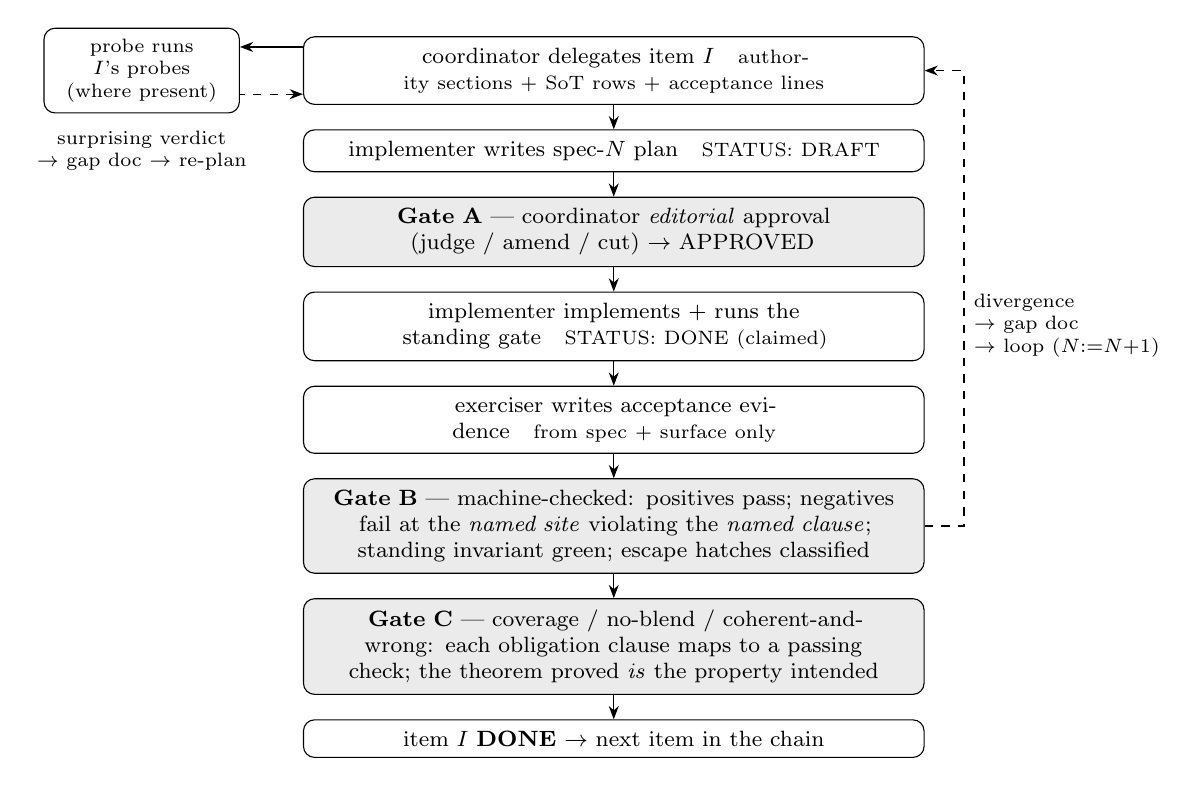
\begin{tikzpicture}[
  node distance=3.1mm,
  >={Stealth[]},
  box/.style={draw, rounded corners, align=center, inner sep=4pt, text width=76mm, font=\footnotesize},
  gate/.style={box, fill=black!8},
]
\node[box]            (co)   {coordinator delegates item $I$\quad{\scriptsize authority sections + SoT rows + acceptance lines}};
\node[box,below=of co]   (plan) {implementer writes spec-$N$ plan\quad{\scriptsize STATUS: DRAFT}};
\node[gate,below=of plan] (ga)  {\textbf{Gate~A} --- coordinator \emph{editorial} approval (judge / amend / cut) $\to$ APPROVED};
\node[box,below=of ga]   (impl) {implementer implements + runs the standing gate\quad{\scriptsize STATUS: DONE (claimed)}};
\node[box,below=of impl] (exer) {exerciser writes acceptance evidence\quad{\scriptsize from spec + surface only}};
\node[gate,below=of exer] (gb)  {\textbf{Gate~B} --- machine-checked: positives pass; negatives fail at the \emph{named site} violating the \emph{named clause}; standing invariant green; escape hatches classified};
\node[gate,below=of gb]  (gc)  {\textbf{Gate~C} --- coverage / no-blend / coherent-and-wrong: each obligation clause maps to a passing check; the theorem proved \emph{is} the property intended};
\node[box,below=of gc]   (done) {item $I$ \textbf{DONE} $\to$ next item in the chain};
\foreach \a/\b in {co/plan,plan/ga,ga/impl,impl/exer,exer/gb,gb/gc,gc/done} \draw[->] (\a)--(\b);
% probe side-branch off the coordinator, with its own pre-spec loop-back
\node[box,left=8mm of co,text width=22mm,font=\scriptsize] (probe) {probe runs $I$'s probes (where present)};
\draw[->] ([yshift=3mm]co.west) -- ([yshift=3mm]probe.east);
\draw[<-,dashed] ([yshift=-3mm]co.west) -- ([yshift=-3mm]probe.east);
\node[font=\scriptsize,align=center,below=1mm of probe] {surprising verdict\\$\to$ gap doc $\to$ re-plan};
% Gate B divergence loop-back
\draw[->,dashed] (gb.east) -- ++(5mm,0) |- (co.east)
  node[pos=0.22,right,align=left,font=\scriptsize]{divergence\\$\to$ gap doc\\$\to$ loop ($N{:}{=}N{+}1$)};
\end{tikzpicture}
\caption{The per-item pipeline. Gate~A is the coordinator's
\emph{editorial} approval of the plan (judgment, not machine output); Gate~B is
machine-checked acceptance; Gate~C is the coherent-and-wrong / no-blend coverage
guard. Forward motion through the status handshake; backward motion through gap
documents; \emph{done} defined only by the gates.}
\label{fig:pipeline}
\end{figure}

Three gates structure each item (Figure~\ref{fig:pipeline}). Gate~A validates the property or
plan against the upper bound. One honest asymmetry belongs here, not only in Limitations:
a single loop's Gate~A is the coordinator's \emph{editorial} judgment, and within that loop it is
the one actor nothing squeezes --- no disjoint $(U,L)$ pair is held over it. The soft half would
then funnel through an un-squeezed judge. The construction's answer is to \emph{nest}: wrap the
loop in an outer squeeze whose monitor holds a disjoint $(U,L)$ pair over the inner loop's
coordinator and its soft outputs --- Gate~S (below) generalized from one learned skill to the
whole loop, the \emph{squeeze-monitoring-a-squeeze} pattern. Nesting \emph{closes} the inner
loop's Gate~A: that coordinator is now squeezed from outside, by an authority it does not hold.
Both our applications are built this way --- the four seeded instances
(Section~\ref{sec:archetypes}) are squeezed by the outer
loop that produced this manuscript (\S\ref{sec:reflexive}), and the \code{lace} application nests
\code{creusot-sl} inside a monitoring loop, \code{creusot-monitoring} (\S\ref{sec:realworld}) ---
and the recursion \emph{must} terminate in a \emph{human}. This is the whole answer to the regress
objection (\emph{who squeezes the squeezer?}): a stack of automated monitors only relocates the
un-squeezed editorial judgment one level up --- it can never close it. Only a person outside the
entire construction can, and the strategy \emph{requires} that one does. A human must end the
nesting, full stop (\S\ref{sec:reflexive} reports exactly this terminal squeeze working:
a Gate-A caption error every internal gate missed and an outside reviewer caught). That terminus
is bounded, which keeps it both tractable and disjoint: the human does not re-verify the artifact
from scratch --- the hard gates have already settled the executable side --- but adjudicates only
the soft-side residual, the \emph{delta} between what the upper bound claims and what the lower
bound established, holding $U$ and the gate record without having produced the work they judge. So the soft
side is closed by disjoint authority all the way up to that mandatory human terminus; the \emph{hard} half
(Gate~B/C against the executable lower bound) is closed mechanically, \emph{by construction}, with
no judge in the loop at all. Gate~B is machine-checked acceptance, including
a \emph{standing
invariant} rerun after every item --- in our instances \emph{total additivity}: byte-identical
output for every pre-existing input, re-confirmed and determinism-checked --- which turns
regression into a definitional impossibility (``if your change alters an existing output, your
change is wrong by definition''). Gate~C is the coverage guard against \emph{coherent-and-wrong}:
each obligation clause maps to a specific passing check, and the theorem actually proved is
checked to be the property intended. Where external ground truth exists Gate~C is
machine-checked; where it does not it is defended by author independence
(Section~\ref{sec:archetypes}).

A fourth gate operates on a different cadence. \textbf{Gate~S} (\emph{skill
consistency}) fires whenever the loop \emph{accumulates} a learned skill --- a soft heuristic an
actor consolidates from its own caught errors. Because that actor shares the skill's blind spot,
the skill is checked by a \emph{monitor squeeze} holding a disjoint evidence base (the loop's own
upper bound and its executable lower bound used as an oracle), which returns \emph{pass}, a
\emph{carve-out} (a narrowing exception that defers to the upper bound where the skill
over-reaches), or \emph{reject}. Gate~S is the no-blend rule of Section~\ref{sec:mechanics}
applied to a loop's own learned outputs --- the per-skill case of the nesting just described, a
squeeze monitoring a squeeze, demonstrated deterministically in Section~\ref{sec:eval}.

\subsection{The disjointness principle, operationally}
\label{sec:disjoint}

Compliance condition (C1) becomes an artifact: the \emph{squeeze table}
(Table~\ref{tab:cast} for the case at hand), written by the coordinator
\emph{before any delegation} and pasted row-by-row into each prompt. An actor learns,
from fresh context, which authorities bind it and, by omission, which evidence it is
denied. The disjointness this enforces is of \emph{evidence}, not of model weights:
the exerciser is independent because the implementation is absent from its context and
it holds an executable oracle, not because it runs on different parameters. Two actors
on the same model but different evidence bases are disjoint here; the same model
judging the same context is not.
Section~\ref{sec:underspec} measures that same- and same-provider cross-model casts ship identical
errors, so --- in the only family we could test --- it is the independent executable oracle, not model
diversity, that carries the gate (a single cross-provider model corroborates the shared blind
spot while partially decorrelating; a powered multi-provider replication remains owed,
\S\ref{sec:limitations}). Disjointness and the oracle do two distinct jobs, and we keep them
distinct: disjointness of \emph{evidence} removes the \emph{possibility} of anchoring --- the
structural guarantee, and the only defense where no oracle exists (Archetype~B) --- while the
\emph{executable lower bound} is what \emph{catches the residual} correlated error in the cases
we measured. The live finding of \S\ref{sec:underspec} speaks to the second: where an oracle
exists, model-disjointness alone does not catch the shared blind spot; the oracle does. The
structural precondition (disjointness) and the catcher (the oracle) are complementary, not competing.
Balance then comes from asymmetry: the implementer can produce
something coherent-and-wrong, but the exerciser, authored from the property alone, cannot be
fooled by the same blind spot; the exerciser could write a vacuous test, but Gate~B demands the
negative fail at a named site violating a named clause; the property author could over-reach,
but expressibility-from-below rejects undischargeable claims; the coordinator could be tempted
to ship, but the gates are machine output it cannot edit. Correctness is the fixed point
satisfying all squeezes at once: the catchability of condition~(C2), which
Section~\ref{sec:synthesis} makes measurable rather than asserted.

% ===========================================================================
\section{A Real-World Application: Trustworthy Proofs (and Real Bugs) in a UEFI Bootloader}
\label{sec:realworld}

We open with the paper's headline real-world result: the strategy applied \emph{unchanged} to an
\emph{external} codebase the authors did not write --- Canonical's \code{lace} UEFI bootloader
framework. The loop proved \ResRWRobust{} input-facing functions robust and surfaced
\ResRWBugsNum{} real, reproducible security defects on a pre-OS attack surface ---
\emph{natural} coherent-and-wrong in production code, direct evidence the target failure occurs in
the wild. The squeeze-specific contribution here is \emph{trustworthy proofs}: the disjoint
faithfulness gate makes a proof trustworthy \emph{by construction}, so a fabricated ``proof'' (code quietly
edited to pass) cannot survive its strip-and-recompile check (\S\ref{sec:realworld-loops}). \emph{Finding} the defects is a
result the underlying deductive verifier delivers, not a squeeze-specific one. This is a
\emph{case study}, not the controlled comparison of Section~\ref{sec:eval}; read it for existence
and reach, not an efficacy rate. The construction is the one already defined (the cast and gates of
Section~\ref{sec:strategy}), instantiating the terrain archetypes formalized next
(Section~\ref{sec:archetypes}). The complete artifacts, issue reports, and per-function verdicts
are in the supplementary material under \code{real-use-case/}.

\subsection{Materials and the two loops}
\label{sec:realworld-loops}

\textbf{Rust and Creusot.} Rust's ownership discipline rules out use-after-free and data races
in safe code, but \emph{not} the failure classes that matter for a parser of hostile input:
integer overflow (a panic in debug, a \emph{silent wrap} in release), out-of-bounds indexing,
unsigned subtraction underflow, and unbounded recursion (a native stack overflow). In a
bootloader --- pre-OS, no sandbox, parsing data it does not control (a PE (Portable Executable)
image on the EFI System Partition (ESP), a partition table on any disk, a \code{grub.cfg} on any
scanned filesystem)
--- each is a pre-Secure-Boot-measurement denial of service (DoS), or on a release-mode silent wrap a
wrong-length or wrong-sector hazard in the loader path. The executable lower bound is
\textbf{Creusot} \citep{denis2022creusot}, a deductive verifier translating Rust through Why3
\citep{filliatre2013why3} to SMT (satisfiability-modulo-theories) solvers, with specifications in its Pearlite contract language.
The single move that turns it into a bug-finder is to \emph{specify a parser for total
robustness}: no panic, overflow, or out-of-bounds read for \emph{any} input, with no
input-restricting precondition. An unproved verification condition is then not a proof failure
but a pointer at a real, reachable bug, and the guard that discharges it is the fix.

\textbf{The two nested squeeze loops.} The application is built as two loops instantiating the
strategy of Section~\ref{sec:strategy}. \emph{\code{creusot-sl}} verifies one file: its upper
bound is an external requirement made precise as Pearlite, its lower bound is \code{cargo
creusot} discharge plus tests plus a mutation probe, and it runs the canonical cast with the
implementer (Table~\ref{tab:cast}) recast as an \emph{annotator} that adds proof scaffolding but
never rewrites behaviour. \emph{\code{creusot-monitoring}} verifies a whole crate by driving a
\code{creusot-sl} sub-loop per file and monitoring its soft outputs: a loop monitoring a loop,
the Gate~S pattern of Section~\ref{sec:mechanics}, with the mission guidance as upper bound and
\code{creusot-sl}'s machine verdicts as lower bound. ``Applied unchanged'' means the topology
and squeeze are fixed while the gate \emph{materials} are rebuilt per terrain. Two
specializations carry the soundness. A \emph{faithfulness gate} re-derives the barrier
mechanically: stripping every annotation must reproduce the \emph{byte-identical} original source
(we verify \code{lace}, we do not rewrite it), so a fabricated proof is caught and reverted
automatically. What makes this the squeeze rather than ordinary annotation hygiene is \emph{who}
enforces it: not the prover choosing not to edit the code (a discipline it can lapse from, or be
prompt-injected out of), but a disjoint mechanical check the prover cannot influence and that runs
regardless --- the producer of a proof is structurally barred from also certifying its faithfulness. A security \emph{Gate~C} rejects any \code{\#[requires]} that narrows the
adversarial input domain --- the dominant coherent-and-wrong being a green proof that quietly
\emph{assumed the attacker away}, worthless when malformed input is the whole point. As in the
constructed instances the barrier is physical: each \code{creusot-sl} runs as a sub-agent, so a
judge sees only returned verdicts, never a producer's rationale.

\subsection{Results}
\label{sec:realworld-results}

The loop was first hardened, unsupervised, on a \emph{warm-up corpus} --- Creusot's own test
suite, stripped of all annotations and reduced to the \ResRWCorpusFiles{} files that compile as
plain Rust --- which it re-annotated and proved (\ResRWCorpusProved{} proved,
\ResRWCorpusPartial{} partial, \ResRWCorpusFailed{} failed, \ResRWCorpusTrivial{} trivial),
confirming the loop runs at crate scale before it was pointed at \code{lace}.

This is where the squeeze, not Creusot, earns its keep. The \code{lace} defects below surfaced
as Creusot verification conditions a lone agent running adversarial total-robustness specs might
also have found; \emph{finding} them is a Creusot result, not a squeeze-specific one. What the
squeeze adds is that the proofs are \emph{trustworthy by construction}. An agent that ``proves''
code by quietly editing it is the coherent-and-wrong failure exactly, and only a disjoint check
catches it: the faithfulness gate strips every annotation and requires the original source back
byte-for-byte, so such a fabricated proof cannot survive --- mechanically, unattended, with no
detection rate to tune or report.

Pointed then at the \code{lace} parsers of untrusted boot-time input, the loop carried every
input-facing parser function to a verdict, with this disposition: \ResRWRobust{}
\textbf{robust} (\ResRWRobustPOne{} on the disk/ESP surface, \ResRWRobustPTwo{} on the
peripheral/firmware surface), \ResRWBugsNum{} \emph{defect-bearing}, \ResRWPartial{}
\emph{partial}, and ${\sim}$\ResRWBlocked{} \emph{blocked} by verifier modeling gaps
(an approximate count --- the blocked files are not cleanly function-decomposed). That is
about \ResRWDistinctFns{} distinct functions, the recursion defect (\code{ISSUE-4}) lying
inside one of the blocked files and so counted in both the defect-bearing and blocked tallies.
Each robust function is provably free of panic,
overflow, and out-of-bounds access for \emph{any} input, under totality-only
extern-specifications and with no \code{\#[trusted]} or \code{assume!} on any
verified logic. The loop found \ResRWBugsNum{} real defects, each with a minimal
adversarial input and a one-line fix (filed as \code{ISSUE-1..4} under
\code{real-use-case/lace-issues/}; five distinct hazards, the PE section-alignment
site carrying two): a subtraction underflow in the PE parser
(\code{e\_lfanew - 64} on a crafted header), a divide-by-zero and a \texttt{u32}
multiply overflow in PE section alignment, a \texttt{u64} multiply overflow in the
MBR (Master Boot Record) extended-partition walk, and an unbounded recursion in the GRUB \code{submenu}
parser (a stack-overflow DoS). Of the four, \ResRWBugsVC{} surfaced exactly as
verification conditions that would not discharge once the parser was specified for
total robustness; the remaining \ResRWBugsCallGraph{} --- the recursion --- was found
by call-graph analysis, Creusot being blocked on that file. Two arithmetic
defects were reproduced on \code{rustc} 1.96.0 in both debug and release.
Independently, the run re-checked the architecture report's structural claims and
reproduced its \code{unsafe}-site counts exactly (\ResRWUnsafePlatform{} in the
platform crate, \ResRWUnsafeUtil{} / \ResRWUnsafeStubble{} / \ResRWUnsafeSpeedboot{}
in the others).

\subsection{What it does and does not establish}
\label{sec:realworld-scope}

A \emph{robust} verdict buys exactly one thing: that function provably cannot panic, overflow,
or read out of bounds on any input, removing it from the exploitable surface. It is \emph{not} a
full mathematical proof of the \code{lace} codebase, and the experiment makes no such claim.
Robustness is neither functional correctness nor a security property: Secure Boot enforcement,
TPM (Trusted Platform Module) measurement, and correct kernel handoff are firmware/behavioural
properties Creusot cannot
model, and were routed out-of-scope rather than pretended. The \ResRWUnsafePlatform{}
\code{unsafe} FFI (foreign function interface) sites in the platform crate are outside the loop's reach by design ---
\emph{measured} statically (the run reproduced this count exactly), not proven. The
${\sim}$\ResRWBlocked{} \emph{blocked} functions of the disposition above arise from verifier modeling gaps (no
\code{Invariant} for \code{String}, missing \code{\&str}-iterator specifications, recursive-type
rejection), so their safety rests on by-hand argument; the recursion defect itself lives in one
such file. The \ResRWPartial{} \emph{partial} functions are panic-safe with no counterexample
but carry a residual obligation the bundled solvers did not close (SMT incompleteness, not a
bug). The proofs rest on a stated trust base: totality-only extern-specs and a hand-built
faithful harness whose fidelity the faithfulness gate checks but does not eliminate as an
assumption.

Two scope limits bound the contribution itself. First, the \ResRWBugsNum{} defects are real
findings, but the \emph{absence} of further defects in the robust functions is a guarantee only
for those functions under their trust base, not a clean bill of health for the bootloader.
Second, no baseline pipeline was run on the same code, and the run used a single team, provider
family, and toolchain. This is an \emph{existence} result, not the powered efficacy comparison of
Section~\ref{sec:eval}. What it adds beyond the seeded instances is what those could not show:
\emph{natural} coherent-and-wrong defects exist in real, externally-authored code, and a disjoint
executable lower bound surfaces them. It approaches the real-bug study of Section~\ref{sec:eval}
from the deductive-robustness side, complementary to the SWE-bench \citep{jimenez2023swebench}
patch-generation route wired there.

\paragraph{Replication.} A replicating team needs \code{rustc}~1.96.0, the Creusot toolchain, and the
faithfulness gate (\code{verify/}); the strip-and-recompile check rejects any annotation-only edit
\emph{deterministically}, and the \ResRWBugsNum{} defects reproduce against the pinned inputs. What is
confirmed is the gate's verdict, not a particular defect count: the defect-\emph{finding} rode unpinned
LLM agents from one provider family and is logged rather than re-run (full provenance and replication
path, \S\ref{sec:limitations}).

% ===========================================================================
\section{Terrain Archetypes: Where the Truth Lives}
\label{sec:archetypes}

The topology above is invariant; the \emph{materials} of each squeeze are not, and the coordinator's
first act on a new instance is to locate where truth lives. We instantiate the three archetypes as four
executable, reproducible squeezes (Table~\ref{tab:synthesis}): \textbf{A}~tabular analytics and
\textbf{D}~formal proofs in Rocq, both \emph{transcription} on very different lower bounds;
\textbf{B}~a refund agent on \emph{authored authority}; and \textbf{C}~an API contract guard on
\emph{split planes}. Each ran as a coordinator--worker loop of LLM coding agents, measured end-to-end.
Each is a \emph{wiring check} --- we seed an internally-consistent defect designed to violate the
oracle, and the gate catches it --- a wiring check that the construction instantiates on the terrain.

\paragraph{A --- transcription (tabular analytics).}\label{sec:caseD} Upper bound: a machine-parsable
metric handbook. Lower bound: a frozen SQL warehouse plus a signed ledger of
\ResWorkedCertifiedMetrics{} figures that recompute byte-for-byte. A gross-revenue (coherent-and-wrong)
implementer is rejected at Gate~B because the exerciser, holding only the handbook, expected net;
without that disjoint exerciser the wrong number has nothing to fail against --- the no-independent-oracle
regime of the test-oracle problem \citep{barr2015oracle}. Scripts under \code{src/A/} regenerate every
figure.

\paragraph{B --- authored authority (refund agent).}\label{sec:caseE} The hardest terrain: no external
authority exists, so the lower bound (a frozen REST app plus a signed archive of \ResBArchiveCases{}
adjudicated decisions) shares the policy author's provenance. The honest reading is an \emph{asymmetric}
guarantee --- the squeeze removes conversational anchoring (a \emph{necessary} condition), but, lacking
an external oracle, cannot supply sufficiency; it reduces to author independence (the Fagan/Cleanroom
move) plus that anchoring guarantee, and no more. Seeded policy-violating bots
\citep{perez2022ignore,greshake2023injection} are caught by the spec-only exerciser via a REST lockpoint
admitting only \texttt{REIMBURSE}/\texttt{DENY}/\texttt{ESCALATE}; the genuinely \emph{live} refund
result is \S\ref{sec:underspec}.

\paragraph{C --- split planes (API contract guard).}\label{sec:caseF} Correctness divides across a
document plane (OpenAPI schema) and a runtime plane (live server); the characteristic failure is
\emph{blending} --- compliant docs masking broken runtime. The exerciser derives \ResCTestCases{}
conformance cases from the schema alone and runs them against the live server
\citep{atlidakis2019restler}; seeded clause-violating servers (auth skip, leaked id, raw traceback) are
caught by the no-blend cross-check, which holds the two planes independent rather than letting one stand
in for the other.

\paragraph{D --- transcription, deductively (Rocq proofs).}\label{sec:caseG} The link needs no
\emph{runnable} oracle: here the hard truth is type-checking. A textbook exercise is transcribed into a
formal statement and discharged in Rocq (formerly Coq); the gate is the kernel plus an axiom audit
(\code{Print Assumptions}) rejecting any \code{Admitted} escape, with a code-blind exerciser writing
false mutations. A vacuous or adjacent-property proof is rejected --- the same construction over a
deductive ground truth, where independence is enforced rather than measured.

\subsection{Synthesis: one topology, four materials}
\label{sec:synthesis}

The four instances make the paper's central structural claim concrete: the loop topology is invariant
while the \emph{materials} of each squeeze are rebuilt per terrain (Table~\ref{tab:synthesis}). Across
\ResNTerrains{} instances over all \ResNArchetypes{} archetypes the construction instantiates end-to-end
and its gate fires on each seeded coherent-and-wrong. We report no barrier-on/off detection rate here: in the one case the
off-condition was run with live agents (the pilot of \S\ref{sec:eval}) the exerciser caught the defect
\emph{regardless} of the barrier, because it derives its acceptance test from the spec, not the code.
The barrier would earn its keep only where a judge could otherwise \emph{anchor} to an implementation it
sees --- and even there its measured outcome effect was null (\S\ref{sec:eval}); on spec-derived checks
it changes nothing. The cross-instance counts regenerate from each terrain's evidence
(\code{verify/synthesis.py}), not hand-typed.

\begin{table}[t]
\centering\small
\begin{tabularx}{\textwidth}{@{}>{\raggedright\arraybackslash}p{2.2cm} Y Y Y Y@{}}
\toprule
 & \textbf{A --- transcription} & \textbf{B --- authored authority} &
\textbf{C --- split planes} & \textbf{D --- transcription (deductive)} \\
\midrule
Use case & tabular analytics & autonomous refund agent & API contract guard &
formal proofs \\
\addlinespace
Upper bound made of & a metric handbook & an authored refund policy & an API
governance manifest & a textbook manifest \\
\addlinespace
Lower bound made of & a signed SQL warehouse + baseline ledger & a REST app + a
signed decision archive & an OpenAPI document + a live server & the Rocq kernel +
axiom-audited proofs \\
\addlinespace
Dominant failure & stale / over-claimed number & manipulated decision &
blended planes (docs mask runtime) & vacuous / wrong theorem \\
\addlinespace
Load-bearing gate & Gate~B + total additivity & coherent-and-wrong guard
(exerciser independence) & no-blend cross-check & kernel + axiom audit \\
\bottomrule
\end{tabularx}
\caption{The four executable instances over three terrain archetypes (A and D both
transcription): one invariant topology, different materials, a different gate carrying the
soundness per terrain. We report no seeded barrier-on/off detection rate (see \S\ref{sec:synthesis}).}
\label{tab:synthesis}
\end{table}

Each archetype places the soundness load on a different gate (Table~\ref{tab:synthesis}): transcription
on Gate~B + total additivity, authored authority on the coherent-and-wrong guard defended by exerciser
independence, split planes on the no-blend cross-check, the deductive instance on the kernel's axiom
audit --- one topology shifting its weight to local materials.

% ===========================================================================
\section{A Live-Model Failure Mode: Underspecification and Contradiction}
\label{sec:underspec}

The seeded instances above test the machinery on \emph{specified} tasks. The more interesting
live failure appears where the upper bound is a genuine \emph{soft} truth the model must
resolve --- \emph{underspecified} (it leaves cases implicit) or \emph{self-contradictory} (its
own clauses, or two authorities it cites, disagree) --- the failures capable models do
\emph{not} reliably resist. This is the paper's second live result, beside the real-world
defects of Section~\ref{sec:realworld}; we state it here and give its measurement apparatus with
the evaluation protocol (Section~\ref{sec:eval}).

Manipulation is a wall capable models resist unaided; an \emph{underspecified} upper bound is
not. An exploratory probe (LLM sub-agents, weak to strong; logged under
\code{verify/reports/live/}, non-deterministic, so \emph{not} gated) gave each instance only its
soft bound on cases it leaves implicit, scored against the executable oracle. A control isolates
signal from artifact: with the model allowed to \emph{reason}, three of the four surfaces
\emph{vanish} on these \emph{thin} specs --- on analytics, the API guard, and proofs the strong
model scores perfectly. But thinness, not the terrain, did that work: re-armed as soft truths
that carry a defect, analytics and the API guard make capable models err again
(\emph{Contradiction, not only silence}, below). Proofs --- the deductive instance~D --- are
deliberately \emph{not} re-armed, and the live floor measured below is therefore A, B, and C only:
D has no \emph{soft} upper bound to contradict. Its bound is a \emph{formal} specification and its
gate a proof checker, so ``coherent-and-wrong'' on D is a fabricated or vacuous proof, which its gate
rejects \emph{deterministically} --- the Rocq kernel plus an axiom audit (\code{Print Assumptions}) and
code-blind mutations (\S\ref{sec:caseG}), the deductive cousin of \code{lace}'s strip-and-recompile
faithfulness check (\S\ref{sec:realworld}) --- a yes/no construction check, not a stochastic divergence
with a rate that varies by capability or provider. D's evidence is the gate firing by construction; it
has no capability curve to draw. The refund agent is different: its surface
\emph{survives and grows} under reasoning, and across the tiers we ran it showed
\emph{no monotone improvement with capability}, the strongest model diverging as often as the weakest
(about a quarter of a balanced gap pool), with three cases missed by \emph{every} tier (one draw per
cell; the powered qwen ladder in Figure~\ref{fig:floor} repeats it). The oracle encodes defaults the
prose never states (a delivered order it never rules on), and a capable model fills the gap with its own
\emph{coherent} policy that diverges from the answer key. We do not claim the model is \emph{wrong} ---
the underspecified bound leaves the reading open --- but that the squeeze performs
\emph{latent-underspecification surfacing}: it exposes a spec gap self-evaluation cannot see and routes
it to the policy-owner for adjudication.

A pipeline comparison on the same cases quantifies what that gate earns. Scoring each
\emph{shipped} decision against the key: raw generation and self-authored tests ship the
coherent-and-wrong on most gap cases; self-critique halves it; a same-context critic and an
LLM-judge cut it to about a sixth; only the squeeze's \emph{executable oracle} ships none. What
every model-based check passes, and the oracle alone catches, is the model-\emph{consensus}
reading (a damaged or changed-mind item refunded where the authored decider escalates). The
nuance: a same-model compliance check already catches the clause-derivable errors, so the gate's
irreducible value is the executable lower bound, not model disjointness. A same-provider cross-model
cast confirms this within the family --- across every implementer/exerciser tier pairing, same- and
same-provider cross-model alike, the consensus errors ship \emph{identically}. A single \emph{cross-provider}
model (a 27B Qwen, Alibaba --- independent pretraining; logged, not gated) gives a first data
point beyond the family: it errs at the same \(25\%\) rate as the haiku and opus casts
(\(3/12\), stable across repetitions) and shares the blind spot on the pure unstated-default
cases (a delivered order; an already-refunded one), so the surface is not Anthropic-specific. But the correlation is only \emph{partial} ---
the Qwen reads one ``manager'' case correctly where every Claude tier escalated, and newly caves
on a high-value new account. A genuinely independent provider thus decorrelates on part of the
surface: direct, if preliminary, evidence for the limit of \S\ref{sec:limitations}. This is the
Knight--Leveson correlation, measured \emph{within one provider family} and probed once across
providers; a fully powered, multi-provider version is future work.

\paragraph{Contradiction, not only silence.} A soft truth fails the model not only by
\emph{silence} (underspecification) but by \emph{self-contradiction}, and contradiction does not
wash out with capability. We re-armed the analytics handbook (A) and the API manifest (C) with
\emph{authority-vs-authority} defects --- two named, real authorities that genuinely disagree:
for A, ASC~606 (the US revenue-recognition accounting standard) net-revenue against a binding
finance directive reporting gross, a GA4 (Google Analytics~4)
``active user'' against a product-council directive excluding logins, and a point-in-time
data-governance standard against a GDPR (General Data Protection Regulation) Art.~17 erasure
directive; for C, RFC~7396 (an IETF Request for Comments; its merge-patch
\code{null} \emph{deletes} the member) against a vendor ``governance override'' (Zalando's
guideline) that ignores it. The executable lower bound adjudicates each; we measured how often a live model handed only the
contradictory spec lands elsewhere, repeated across a qwen capability ladder (4B/9B/27B; $n{=}24$ per
contested fork) and a three-provider panel (Alibaba \code{qwen3.6:27b}, Google \code{gemma4:31b}, Meta
\code{llama4}; logged under \code{verify/reports/live/}, not gated).

Figure~\ref{fig:floor} is the result. On the forks where \emph{both} authorities are genuinely
legitimate the error is a \emph{floor}: the GA4 \code{active} fork (and the unstated-default refund on
B) is missed at near-$100\%$ at \emph{every} size, and the three-provider panel reproduces this
identically ($24/24$, $24/24$, $8/8$ across all three --- three providers on constructed cases, not
invariance in a broader sense).

\paragraph{Scaling makes the contradiction worse.} The GDPR-erasure \emph{survivorship} fork is the
sharper finding: its error \emph{rises} with capability ($0.54\to0.83\to1.00$ across the qwen ladder),
the larger models more confidently following the erasure override into the wrong answer. So on a
genuinely-balanced contradiction, capability is not merely unhelpful but actively harmful. Capability
settles only the \emph{decidable} conflicts (a sloppy
\code{net}/gross directive, an inconsistent window), and there genuine model diversity \emph{spreads
out} rather than agreeing (on \code{net}, llama resists $16/24$ where qwen and gemma err $24/24$; on the
patch-null override gemma $16/16 >$ qwen $12/16 >$ llama $7/16$). On the genuine contradictions it is
powerless and the disjoint executable lower bound is the only adjudicator. (On instance~B the floor fork
\code{delivered\_default} ``diverges'' from the authored archive rather than being ``wrong'': B's archive
shares the policy-owner's provenance, so this is underspecification \emph{surfaced}, not detection
against an independent oracle, which B lacks.) These are deliberately constructed defects --- an
existence demonstration of the failure mode and its capability profile, not a frequency over real specs.

\begin{figure}[t]
\centering
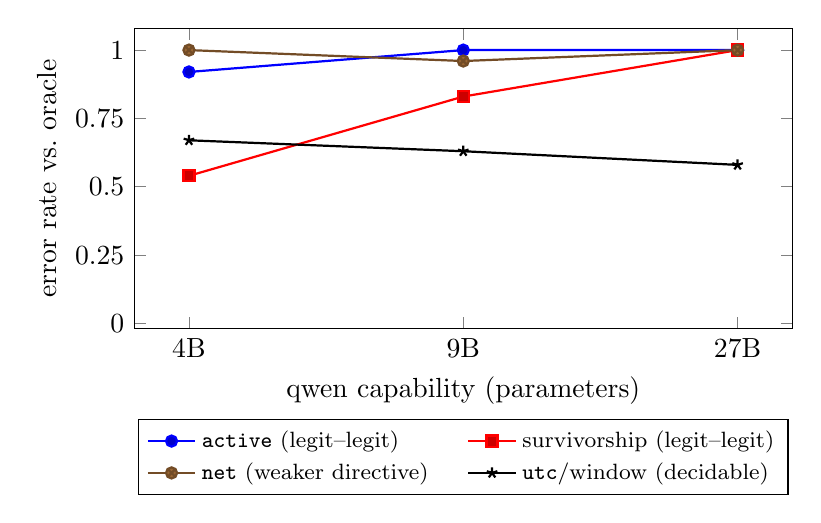
\begin{tikzpicture}
\begin{axis}[
  width=0.82\linewidth, height=5.4cm,
  xlabel={qwen capability (parameters)}, ylabel={error rate vs.\ oracle},
  xtick={1,2,3}, xticklabels={4B,9B,27B},
  ymin=-0.02, ymax=1.08, ytick={0,0.25,0.5,0.75,1.0},
  legend style={at={(0.5,-0.30)}, anchor=north, legend columns=2, font=\footnotesize,
    /tikz/every even column/.append style={column sep=12pt}},
  legend cell align=left,
  every axis plot/.append style={thick, mark=*},
]
\addplot coordinates {(1,0.92)(2,1.0)(3,1.0)};   \addlegendentry{\code{active} (legit--legit)}
\addplot coordinates {(1,0.54)(2,0.83)(3,1.0)};  \addlegendentry{survivorship (legit--legit)}
\addplot coordinates {(1,1.0)(2,0.96)(3,1.0)};   \addlegendentry{\code{net} (weaker directive)}
\addplot coordinates {(1,0.67)(2,0.63)(3,0.58)}; \addlegendentry{\code{utc}/window (decidable)}
\end{axis}
\end{tikzpicture}
\caption{On a genuinely-balanced contradiction, scaling makes the error \emph{worse}: the GDPR-erasure
\emph{survivorship} fork rises $0.54\!\to\!1.00$ with model capability --- the larger model follows one
authority off the cliff more confidently. Error rate vs.\ capability on contradiction instance~A, across
the qwen ladder (4B/9B/27B; $n{=}24$ per fork; the two 27B generations pooled at 27B). The other
genuinely-balanced fork (\code{active}) is a near-$100\%$ floor throughout; the decidable \code{utc} fork
stays low. At flagship scale the three-provider panel (Alibaba/Google/Meta) reproduces the balanced-fork
floor at $100\%$; on the weaker-side forks the providers spread out (gemma most override-compliant, llama
least). Underlying counts in \code{verify/reports/live/}. All values are point estimates ($n{=}24$ per
fork per size) with no confidence intervals; the replicable target is the qualitative trend---the
\emph{survivorship} fork rising with capability, the genuinely-balanced floor forks staying near
$100\%$---not the exact decimals.}
\label{fig:floor}
\end{figure}

\paragraph{Replication.} A replicator needs the \code{build\_cases()} probes
(\code{src/\{A,B,C\}/ground-truth/}) scored against each instance's executable oracle. The confirmed
target is the \emph{floor}, not the per-draw decimal: the GA4 active-user contradiction and the
unstated-default refund are near-$100\%$ across every model we ran (Claude haiku--opus, qwen 4B--27B,
gemma, llama), while the GDPR-erasure survivorship fork is near-$100\%$ at flagship scale and rises with
capability (lower on the smallest qwen). The exact rate is non-deterministic and logged, not gated (full
path, \S\ref{sec:limitations}).

% ===========================================================================
\section{The Reflexive Case Study: This Paper as a Squeeze Loop}
\label{sec:reflexive}

This manuscript was produced under the strategy it describes: its upper bound is the peer-reviewed
literature (each source recorded before it may be cited), its lower bound the \ResReflexTerrains{}
executable instances and their harnesses, and \emph{done} is the claim ledger re-derived, not the
authors' satisfaction. The point of interest is what that process caught in \emph{our own} claims before
the paper shipped: \ResReflexDefects{} coherent-and-wrong or over-claim defects (\ResReflexDefectsLit{}
on the literature plane, \ResReflexDefectsEvid{} on the evidence plane) --- a comparative overstated, a
finding misattributed, a figure crediting the wrong source, an abridged quotation shown as verbatim ---
each fluent and correct-looking, each found by re-deriving the claim from its source, not by re-reading
the prose (all \ResReflexDefects{} enumerated in Appendix~\ref{app:reflexdefects}). This is the global
story turned inward: coherent-and-wrong is not a property of implementations alone; soft-side editorial
claims fail the same way, and only re-derivation from an independent source catches them.

The honest limit is in the strategy's own terms: a single team is not independent of itself, so the
gate's independence was only \emph{approximated} --- a disjoint same-provider sub-agent, a cross-provider
framing judge, and the human peer reviewer as the mandatory terminus that closes the un-squeezed Gate~A
(who caught \ResCalibExternalCatches{} defect our own gates missed). It is an $n{=}1$ illustration of the
mechanism catching its target, not a controlled result; the approximation's mechanics are in
\code{paper-impl.md}.

% ===========================================================================
\section{Proposed Evaluation Protocol}
\label{sec:eval}

\emph{This section is a protocol proposal with mostly-null pilots, not a completed
evaluation.} The strategy's efficacy is \emph{non-linear}, so these null pilots are a
\emph{boundary condition}, not a shortfall: on small, well-specified tasks the
per-implementation error base rate is near zero, leaving the barrier nothing to catch and no
marginal value to add; it becomes strictly necessary only on \emph{contested} soft specs ---
underspecified or self-contradictory --- where capable models diverge and added capability does
not fix it (\S\ref{sec:underspec}). The deterministic mechanism is established on the four executable instances
(Section~\ref{sec:synthesis}), but it has not been evaluated under \emph{controlled,
comparative} conditions. This section fixes the hypotheses and measurements we expect to matter,
operationalizes them as a runnable harness (\code{verify/\allowbreak eval\_protocol.py}), and
reports what we have so far been able to run. The four hypotheses are: \textbf{H1}, disjointness
lowers the coherent-and-wrong rate versus shared context; \textbf{H2}, physical barriers reduce
evidence--implementation coupling and catch more seeded defects; \textbf{H3}, the Gate-A amendment
rate predicts the downstream gap rate; and \textbf{H4}, protocol overhead amortizes on long
regression horizons. The supporting evidence we have today is
exploratory: one \emph{live} result (instance~B's underspecified cases diverge from the authored archive
in a way added capability does not fix, surfaced only by the executable lower bound --- coherent-and-wrong
in the \emph{surfacing} sense of \S\ref{sec:underspec}, not adjudicated against an independent oracle,
which B lacks; below) and one
\emph{reflexive} illustration (this manuscript had \ResReflexDefects{} coherent-and-wrong or
over-claim defects caught before submission, \ResCalibExternalCatches{} only by external review;
Section~\ref{sec:reflexive}) --- existence proofs that the gate catches the target failure, not
rates.

\paragraph{Protocol status.} Of the harness's \ResEvalHypTotal{} hypotheses,
\ResEvalHypMeasured{} (H2) is \emph{partially} demonstrated on the four instances as a
consistency check: its seeded-detection half shows only that the gate fires on each terrain's
seeded coherent-and-wrong (a wiring check; we report no barrier-on/off detection rate,
\S\ref{sec:synthesis}), while its \emph{coupling} half is only illustrative and the barrier-off
delta remains future work. The remaining \ResEvalHypPending{} (H1, H3, H4) and
\ResEvalConfigsPending{} comparative configurations are wired as explicit stubs reporting their
prerequisites (a real LLM-agent pipeline, a matched-difficulty suite, cross-model casts,
repetitions, a significance test); no numbers are fabricated. The nulls confirm only that the
seeded tasks are too easy to elicit coherent-and-wrong; the live evidence below comes from the
contested regime instead.

\paragraph{What we have run.} The comparative configurations were executed as pilots with LLM
subagents, and all return the same null. With a seeded coherent-and-wrong implementation, the
exerciser caught the defect on all \ResPilotTasks{} tasks whether shown the specification alone
or also the code: it tested against the spec, not the code. Across self-authorship, a weaker
model, and a pre-committed \ResStudyImpls{}-implementation study over three tiers on harder
tasks, the implementers produced almost no bugs (\ResPilotTwoBuggy{}, \ResPilotThreeBuggy{},
\ResStudyBuggy{}; McNemar $p=\ResStudyP{}$ on the last --- vacuous, no discordant pairs), so no
self-authored defect existed to miss. The obstacle is not statistical power but a near-zero
per-implementation error rate: current models reliably get small, well-specified functions
right. We report these nulls rather than hunt task space for an effect. The strategy's value is
in any case a \emph{guarantee} --- the barrier removes the \emph{possibility} of anchoring;
these results bound only how often it is realized.

\paragraph{A comparative baseline on defective soft specs.} The near-zero rate is a property of
\emph{thin, well-specified} tasks, not of the strategy: a task with one plausible reading leaves
a capable model nothing to get coherently wrong. When the upper bound is instead a genuine soft
truth carrying a defect --- an underspecified gap (B) or an authority-vs-authority contradiction
(A and C, \S\ref{sec:underspec}) --- live capable models do err, at a nonzero rate only the
executable lower bound catches. Measured across Claude tiers (weak/mid/strong; logged, not gated),
the per-instance error against the oracle was, on the contradiction-armed specs at \emph{five} draws
per case, A $46/75, 25/75, 40/75$ (non-monotone, with the two both-authorities-legitimate
forks wrong at every tier) and C a flat $11/90, 12/90, 10/90$; and on the underspecified refund
policy about $3/12$ per tier (\S\ref{sec:underspec}); capability brings no monotone gain on any of
them, and on A's both-authorities-legitimate forks no gain at all. This is the comparative signal the seeded near-zero pilots could not surface.
It is an existence demonstration on \emph{constructed} defects, not a benchmark rate over real
specs; a genuinely multi-provider version remains future work.

\paragraph{Toward a real-bug study.} A controlled comparison against SWE-bench-Lite
\citep{jimenez2023swebench} is wired as a future path; its effect size awaits the per-repository Docker
images and patch-generating endpoint absent from this build.

\paragraph{Mechanism demonstrations (deterministic, not learning results).} Three pieces of
machinery are wired and shown causal on the executable instances, none a live-model claim. (i)~A
\emph{level-up} apparatus enriches the thin upper bound that makes capable models right by
default: a difficulty ladder per terrain plus a pool of graded-subtlety tasks, with the same
detection primitive throughout (an independent re-derivation flagged when a candidate diverges),
exposing a genuine nonzero error surface against a fixed \emph{weak} implementer; random
sampling of the pool also restores a genuine per-cycle trial. (ii)~The squeeze's ``get caught
$\to$ consolidate'' move is wired into each instance: the deciding agent starts from scratch, the
fixed independent exerciser catches each coherent-and-wrong move, and consolidation removes that
error class --- causal (replaying final cycles against an empty store remakes the errors) and
deterministic (byte-identical on re-run); the deductive instance shows the bounded case, where a
residual conceptual-leap wall persists. (iii)~\textbf{Gate~S} (Section~\ref{sec:mechanics})
\emph{squeezes} the accumulated skills themselves: a monitor holding each instance's upper bound
and executable oracle --- a different evidence base than the deciding agent's caught errors ---
audits them in a recomputable check, repairing an over-reaching ``ignore-it'' skill by a
narrowing carve-out that defers to the upper bound. These establish only that the machinery is
wired and causal --- a deterministic loop eliminates exactly the errors it consolidates against;
they are programmatic learners over fixed catalogs, not live models, so a live model's learning
curve remains open. Full per-instance counts are in the supplementary harness.

\paragraph{What a full evaluation would add (not run).} A powered, comparative protocol
--- squeeze-compliant versus shared-context pipelines at matched difficulty, with defect-escape
and coherent-and-wrong rates as outcomes, the stabilizers ablated one at a time, and a human
audit of Gate~C verdicts --- is specified in the supplementary harness but not run here. The
natural-bug route met a near-zero error rate, and the controlled, multi-provider version needs
infrastructure we did not have (per-repository Docker images, a patch-generating endpoint, and
casts spanning genuinely independent providers). We therefore present the \emph{powered} comparison
as specified-but-unrun --- the exploratory pieces above were run.

\paragraph{Isolating the barrier: a clean negative.} Does removing the implementation from a judge's
context change an \emph{outcome}? We ran the experiment that targets this LLM-specific novelty directly,
fixing the judging mode (write the acceptance figure; accept iff a test asserting it passes) and varying
only the test-writer's context across three arms: spec \emph{alone}; spec \emph{and} the defective code;
spec plus a length-matched \emph{unrelated} file (placebo). On the well-specified gross-vs-net seed
(\S\ref{sec:caseD}), across weak/mid/strong tiers at $12$ draws per cell, a draw \emph{escapes} if its
test ratifies the defective code. Escape was $0/12$ in \emph{every} cell, all tiers, all arms: every
judge, \emph{including} those shown the defective code, derived the spec's figure and caught the defect
(several named the code buggy). The barrier moved nothing. We then ran the arms where it \emph{should}
bind --- an \emph{underspecified} spec (where the dominant response was the squeeze-correct one,
\emph{escalate to the policy-owner}, not anchoring) and a \emph{persuasion} soft-side arm (a binding
policy, a clear violation, a compliance-judge shown the agent's fluent self-justification) --- and escape
was $0/12$ there too. Across all arms ($324$ draws) the barrier's outcome-effect is undemonstrated, for
one reason: given an \emph{explicit} authority a capable model follows it (or escalates the gap)
regardless of what artifact-side material sits in its context.

A weaker, cross-provider ladder (qwen 4B/9B/27B, all passing the control probes) tested the one condition
the Claude tiers could not rule out --- a genuinely weaker judge --- and escape stayed $0/10$. Across
$504$ draws over three regimes, two provider families, and the 4B--Opus range, the barrier's
outcome-effect never appeared. We do not read this as the barrier being useless: the anchoring and
sycophancy failures it targets are documented (\S\ref{sec:sota}). But the regime where they would bind
--- a judge following the \emph{artifact} over an \emph{explicit} authority --- is one a clean isolation
excludes: a model that cannot hold the authority fails the control probes (incompetence, not
coherent-and-wrong), and the experiment must \emph{supply} an explicit authority, the very condition
under which a competent judge does not need the barrier. We endorse interpretation (a): for a competent
model---the only kind whose verdict we would trust---the context barrier is structurally present but
empirically redundant, because such a model follows the explicit authority over the artifact whether or
not it can inspect the implementation. We do \emph{not} claim the barrier is inert for weak judges, where
anchoring might bind; we claim it does not change outcomes in the regime that matters. The executable
oracle and the authority, not the context barrier, carry the load in every condition we could
\emph{cleanly} test.

% ===========================================================================
\section{Limitations}
\label{sec:limitations}

We close by bounding what the strategy does \emph{not} establish, worst first. Each names a specific
place where the link between the soft authority and the
executable lower bound is still incomplete --- on its hard side, on its soft side, or in how far
our evidence reaches.

\textbf{The harder failure is the one the oracle cannot see.} The construction is strongest against
an artifact that \emph{violates} the executable lower bound and weakest against its dual --- an
artifact that \emph{satisfies} the hard check while betraying the soft intent (\S\ref{sec:strategy}).
That dual passes the oracle by definition, so catching it falls entirely to Gate~A, the editorial
judgment that is un-squeezed within a single loop and closed only by nesting terminating in a human
(\S\ref{sec:mechanics}). The \emph{by-construction} guarantee therefore covers the catchable half
--- violations of the hard bound --- and not the half often more dangerous in practice: a fluent,
oracle-passing artifact that is quietly wrong about what was wanted. On that half we have disjoint
authority terminating in human review, not a mechanical guarantee. This bounds the whole claim.

\textbf{Cost and latency.} The protocol multiplies agent invocations and adds documentary
overhead. The \emph{structural} cost is fixed by the cast, not the task: each item is handled by
a coordinator, an implementer, an independently-authored exerciser, and the gates, with a plan
document and any gap documents --- structurally a low single-digit multiple of a single-agent pass
(on the order of a handful of role-invocations per item --- the coordinator's delegation and gate
approval, the implementer, and the exerciser --- plus two short documents, before any retries), paid
per item. What that costs in \emph{tokens and wall-clock} needs per-engagement telemetry we have not
yet instrumented. Hypothesis~H4 conjectures, but does not yet show, that this amortizes on
engagements with long regression horizons and not on one-shot tasks. Because current models
rarely produce coherent-and-wrong on the small, well-specified tasks exercised here, the base
rate of the failure the protocol prevents is itself unmeasured; the external application of
Section~\ref{sec:realworld} shows such defects \emph{do} occur in production code, without
measuring their rate. The cost--benefit case rests for now on the literature of
Section~\ref{sec:sota} and the deferred real-bug study (Section~\ref{sec:eval}).

\textbf{Shared priors.} Context barriers remove \emph{conversational} coupling between agents, not the
correlation induced by shared pretraining --- the Knight--Leveson lesson \citep{knight1986independence}
transposed. We \emph{measured} it: same- and same-provider cross-model casts ship the identical
consensus errors, so disjoint \emph{models} do not catch them; only the executable lower bound does
(\S\ref{sec:underspec}). The Knight--Leveson claim proper --- that correlated error survives
\emph{genuine} model diversity --- cannot be settled from within-family data, so we replicated across a
qwen capability ladder (4B/9B/27B) and three genuinely-independent lineages (Alibaba/Google/Meta): on the
genuinely-balanced contradiction forks the floor reproduces at $100\%$ across all three, while on the
weaker, decidable forks the providers \emph{spread out} --- diversity decorrelates only where an oracle
is least needed (Figure~\ref{fig:floor}). This is begun, not powered: three lineages, not dozens
(DeepSeek and OpenAI \code{gpt-oss} could not be run at power on our host). We state the dependency
plainly: where an executable oracle exists the gate rests on the lower bound, which holds regardless of
model correlation; the \emph{distinctive} claim over prover--verifier games --- that disjointness of
evidence buys independence on oracle-free terrains where only model casts disagree --- rests on that
cross-provider replication, which points the predicted way but is not yet powered. We claim the
within-family results and this preliminary multi-provider corroboration, and no more.

\textbf{The coordinator is a single point of judgment at one level.} Gates A and C concentrate editorial
authority; a negligent coordinator degrades the loop even though it cannot silently corrupt
artifacts, since it never touches source. Nesting is the construction's answer (\S\ref{sec:strategy}):
an outer squeeze holds a disjoint $(U,L)$ pair over the inner coordinator, so no level's editorial
judge is the last word --- the recursion \emph{must} terminate at a human (an external reviewer) who squeezes the
top coordinator; automation alone never closes it. This closes the soft-side hole by \emph{disjoint authority} rather than by
construction; what it does not buy is a mechanical, judge-free guarantee on the soft side, which only
the hard executable bound has. \textbf{An executable lower bound is required:} where
none exists, the first work item must build one (probes, goldens), and domains where no cheap
runnable ground truth can be constructed are outside the strategy's current reach.

\textbf{The lower bound can itself be coherent-and-wrong.} The gate rests on an executable
ground truth, but a flaky or mistaken oracle that happens to agree with wrong code is
coherent-and-wrong at the hard bound itself. Total additivity, determinism re-runs, and a
signed baseline mitigate but do not eliminate this, since a test wrong in the same
direction as the code escapes them. The risk is least where the lower bound is a proof kernel,
greatest where it is authored tests, which then deserve the same independence scrutiny as
the implementation.

\textbf{Provenance of the evidence.} The four executable instances are constructed,
deterministic, and small, built by one team operating LLM coding agents: reproducible
end-to-end but not a controlled comparison, so the generalization claim rests on the evaluation
of Section~\ref{sec:eval}, operationalized and piloted but not yet powered (the pilots met a
near-zero natural error rate, leaving the effect size to a real-bug study). The external
\code{lace} application (Section~\ref{sec:realworld}) adds evidence on code the team did not
author, where the strategy found \ResRWBugsNum{} natural defects --- a bug-finding case study
without a matched baseline, nor a full verification of that codebase. One reproducibility gap is
our own: we pin \code{rustc} 1.96.0 for the \code{lace} reproductions, but the LLM agents are
Anthropic Claude models from a single provider family rather than per-run pinned checkpoints.
For the no-improvement-with-capability observation we report a within-family tier gradient, with exact per-run
snapshots in the exploratory logs (\code{verify/reports/live/}); a cross-provider,
dated-checkpoint replication is owed. There is an honest irony to confront: the numbers our
deterministic harness regenerates byte-for-byte are the \emph{seeded} consistency checks --- the
part we explicitly do \emph{not} rest load on --- while the two load-bearing findings
(\S\ref{sec:realworld}, \S\ref{sec:underspec}) are the non-deterministic, unpinned ones.
Reproducibility-by-construction holds for the wiring; the evidence that earns the architecture rests,
for now, on logged transcripts rather than a re-run. \emph{What a replication needs}, consolidated: for
\code{lace}, \code{rustc}~1.96.0 plus the Creusot toolchain and the faithfulness gate (\code{verify/}),
where the strip-and-recompile check rejects any annotation-only edit \emph{deterministically} and the
\ResRWBugsNum{} defects reproduce against the pinned inputs; for the contradiction/underspecification
finding, the \code{build\_cases()} probes (\code{src/\{A,B,C\}/ground-truth/}) scored against each
instance's executable oracle, on the instruction-tuned models we ran (below). The reproducible target is the
\emph{floor}, not the per-draw decimal: the GA4 active-user contradiction and the unstated-default refund
were missed at near-$100\%$ by every tier and provider we ran (Claude haiku--opus; qwen 4B--27B; gemma;
llama), while the GDPR-erasure survivorship fork was near-$100\%$ at flagship scale but \emph{deepened}
with capability (lower on the smallest qwen). So a replicating team should expect those forks missed at a
high rate --- flat with capability for active and the refund default, rising with it for survivorship ---
not a particular number. The non-determinism we cannot pin is the exact rate; the qualitative floor
reproduced on every model we tried.

\textbf{Skill accumulation is shown for programmatic learners, not live models.} The
caught-then-consolidate result (Section~\ref{sec:eval}) is established with \emph{deterministic
programmatic learners over fixed catalogs}, not live LLMs; a live model's learning curve, and how
the deductive instance's deferred conceptual-leap wall is crossed, remain open.

% ===========================================================================
\section{Conclusion}
\label{sec:conclusion}

The squeeze loop strategy is a small number of decisions applied without exception. Hold every
actor between an authority it must answer to and a ground truth it cannot touch; make those authority
pairs \emph{different} for every actor (the \emph{disjointness principle}), so the intersection of all
constraints is the correct deliverable while no single evidence base suffices; route all motion through
editorially approved plans and gap documents; and let machine gates define done, never an agent's
report. What actually \emph{catches} a coherent-and-wrong artifact, in every condition we could measure,
is the executable lower bound --- an independent oracle that runs and returns a verdict, not a smarter
model, not more agents, and not hiding the code from the judge. Disjointness of evidence carries the load
on the one terrain where no such oracle exists (Archetype~B), and elsewhere is the precondition that
catch builds on. Four executable instances over three
epistemic terrains kept this topology fixed and rebuilt the squeeze from local materials each
time: the strategy's portable core, shown by construction. Applied unchanged to an external UEFI
bootloader the authors did not write (Canonical's \code{lace}), the loop proved \ResRWRobust{}
input-facing functions robust and surfaced \ResRWBugsNum{} real security defects --- with the
squeeze-specific guarantee that
the proofs are \emph{trustworthy by construction}, a fabricated proof unable to survive the
faithfulness gate (a case study, not the controlled comparison still owed, Section~\ref{sec:eval}).
The second live finding earns the architecture: on an underspecified or self-contradictory policy
a capable agent supplies its own coherent reading that diverges from the answer key, a divergence
that showed no \emph{monotone} improvement as capability rose and that same- and same-provider
cross-model casts ship \emph{identically} --- only the executable lower bound surfaces it
(Section~\ref{sec:underspec}). Whether the gates shift outcomes
against the natural error rate of strong models is left as a wired but underpowered study, having
declined to manufacture an effect the data did not show. Applied to its own construction, the strategy caught \ResReflexDefects{}
coherent-and-wrong or over-claim defects in this paper's own claims before submission (\ResCalibExternalCatches{}
only by external review) --- a small $n{=}1$
illustration, not a controlled result (Section~\ref{sec:reflexive}). The compact statement we end
on: \emph{give every agent a truth it must answer to and a truth it cannot touch, make those
truths different for every agent, and let convergence --- not anyone's report --- define done.}

% ===========================================================================
\appendix
\section{The coherent-and-wrong and over-claim defects the process caught}
\label{app:reflexdefects}

Section~\ref{sec:reflexive} reports that the paper's own process caught \ResReflexDefects{}
coherent-and-wrong or over-claim defects in its claims before submission
(\ResCalibExternalCatches{} only by external review). We enumerate them here so the claim is
checkable rather than taken on trust. Each is recorded in
\code{verify/manuscript\_defects.tsv} and was found by re-deriving the claim from its source
or artifact, not by re-reading the prose: \ResReflexDefectsLit{} on the literature plane,
\ResReflexDefectsEvid{} on the evidence plane.

\begin{table}[h]
\centering\small
\begin{tabularx}{\textwidth}{@{}l l Y Y@{}}
\toprule
 & \textbf{Plane} & \textbf{Claim as written (coherent-and-wrong)} & \textbf{Correction} \\
\midrule
D1 & literature & a survey comparison stated as ``outperforms'' more strongly than the cited
source asserts & softened to the source's hedged claim \\
\addlinespace
D2 & literature & full reasoning shared across debate rounds attributed to
\citet{irving2018debate} & reattributed to \citet{du2023debate}, the only realization it
holds of \\
\addlinespace
D3 & literature & Constitutional AI described as sharing weights, unscoped & scoped to its
self-critique stage \\
\addlinespace
D7 & literature & Clover's ``passing all checks implies correctness'' stated as fact & restated
as the authors' hypothesis (caught at full-text read) \\
\addlinespace
D4 & evidence & a figure attributed Gate~C to a guide that has only Gates~A--B & provenance
corrected \\
\addlinespace
D5 & evidence & ``all three guides end with this sentence'' --- the three closing sentences
differ & claim removed \\
\addlinespace
D6 & evidence & an abridged agent transcript shown in a verbatim environment & marked as
abridged \\
\addlinespace
D8$^\ast$ & evidence & a figure caption called Gate~A machine-checked; Gate~A is editorial
judgment & caption corrected \\
\bottomrule
\end{tabularx}
\caption{The \ResReflexDefects{} coherent-and-wrong or over-claim defects the process caught in the paper's
own claims before submission. $^\ast$ D8 is the \ResCalibExternalCatches{} the internal gates
missed --- a peer reviewer caught it, the one party with true context independence
(Section~\ref{sec:reflexive}).}
\label{tab:reflexdefects}
\end{table}

% ===========================================================================
\section{Anti-collapse stabilizers}
\label{app:stabilizers}

A \emph{collapse} is any event in which an actor relieves its own squeeze --- severing, at that node, the
link between the soft authority it must answer to and the executable ground truth it cannot touch. The
four executable instances converged on \ref{item:laststab}~rules that block collapse structurally
(Table~\ref{tab:collapse} maps collapse modes to the rule that blocks each). These are \emph{operational
lore} distilled from running the loop, not theorems --- a practitioner checklist, not part of the formal
apparatus of Section~\ref{sec:strategy}.

\begin{enumerate}
\item \textbf{Forbidden moves are load-bearing.} Each role's negative constraints (never edit the
  drivers, never read the diff, never implement a fix, never touch source) keep the squeeze from
  collapsing: any actor allowed to cross roles can relieve its own pressure.
\item \textbf{Information barriers are physical, not honorary.} Separation is enforced by what is in the
  delegation prompt (fresh context, surface and acceptance lines only), not by asking an agent to
  refrain.
\item \textbf{Done is gate-defined, never self-declared.} Done is machine gates passing, witnessed by
  independently authored evidence; self-assessment is never evidence.
\item \textbf{Conservation laws bound the blast radius.} A standing invariant (total additivity; standing
  proof counts; determinism re-runs) is rerun after \emph{every} item, turning regression into a
  definitional impossibility.
\item \textbf{Surprise is routed, never absorbed.} A surprising probe verdict or failing acceptance line
  becomes a gap document; a local workaround silently desynchronizes the workflow's model of reality.
\item \textbf{Pin reality before building on it.} One claim per probe, one minimal experiment, one
  recorded verdict; feasibility proven on a minimal instance before machinery is built.
\item \textbf{Specify the implicit base before extending it.} Transcribe existing de facto behaviour into
  the references before adding anything; verify by independent prediction.
\item \textbf{Editorial approval gates the plan, before code.} The approval must amend, cut, or sharpen;
  a rubber stamp makes the coordinator's upper bound fictional. No source edit from a \code{DRAFT}.
\item \textbf{Honest scope is a deliverable.} Explicit NOT-claims and the classification of every escape
  hatch make what was \emph{not} proven as legible as what was.
\item \textbf{Strictness has a safe direction.} The implementation may be stricter than the authority,
  never weaker; divergence-by-strictness is legitimate, divergence-by-weakness is a bug.
\item \textbf{Sequence by mechanism reuse; parallelize only across independence.} Each item rides
  machinery the previous one hardened; chains are parallel only when they share no evidence base and no
  deliverable.
\item \textbf{Traceability is itself an acceptance criterion.} Every change traces to an approved plan,
  every plan to the gap or authority section that motivated it.
\item\label{item:laststab} \textbf{Where authority is authored, independence is the soundness argument.}
  With no external spec to diff against, the only defense against coherent-and-wrong is that the
  property's author and exerciser never saw the implementation; the design must name this (Gate~C) and
  protect it.
\end{enumerate}

\begin{table}[h]
\centering\small
\begin{tabularx}{\textwidth}{@{}>{\raggedright\arraybackslash}p{3.4cm} Y >{\raggedright\arraybackslash}p{2.3cm}@{}}
\toprule
\textbf{Collapse mode} & \textbf{Symptom} & \textbf{Blocked by} \\
\midrule
Self-judging & implementer edits or authors its own acceptance; tests pass suspiciously fast & 1, 2 \\
Shared evidence & two actors hold identical $(U,L)$ pairs; an error propagates unchecked & (C1) audit \\
Honorary barrier & internals present in the judge's context & 2 \\
Self-declared done & ``the agent reported success'' ends the item & 3 \\
Absorbed surprise & local workaround; the loop's model of reality drifts & 5 \\
Rubber-stamp approval & plans approved verbatim, instantly & 8 \\
Coherent-and-wrong & a valid result proving an adjacent, weaker property & Gate~C; 13 where authored \\
Weakened clause & ``it proves now'' after the obligation was quietly softened & 10 \\
Regression by rationalization & ``that diff is expected'' & 4 \\
Unpinned reality & design built on assumed tool behaviour & 6 \\
Unspecified base & features grown on implicit behaviour & 7 \\
Scope blur & silent over-claiming; unclassified escape hatches & 9 \\
Unsequenced parallelism & parallel chains share an evidence base or deliverable & 11 \\
Orphan change & an edit with no plan, no gap, no authority behind it & 12 \\
\bottomrule
\end{tabularx}
\caption{Collapse modes and the stabilizers that block them. Numbers refer to the list above; (C1) is the
disjointness audit of Definition~\ref{def:compliance}.}
\label{tab:collapse}
\end{table}

% ===========================================================================
\bibliographystyle{plainnat}
\setlength{\bibsep}{3.2pt plus 0.3ex}
\bibliography{references}

\end{document}
